\documentclass[11pt,reqno]{amsart}
%==============================================================
%  Transport and tiling bounds for the affine plank problem on the triangle:
%  new sharp cases, a rigidity theorem, and a normalizer obstruction.
%
%  ACADEMIC-CORRECTNESS POLICY (binding): every Theorem/Proposition/Lemma is
%  either cited (with attribution) or proved in full here. Not-yet-established
%  statements live in Conjecture/Problem/Remark and are never used as proved.
%  SCOPE (honest): this studies the triangle as a CONCRETE body plus method.
%  It is NOT an attack on the general conjecture via Ambrus (whose reduction
%  targets simplices of dimension 2N-1; the triangle is never a target).
%==============================================================
\usepackage{amsmath,amssymb,amsthm,mathtools}
\usepackage{tikz}
\usepackage[margin=1.1in]{geometry}
\usepackage[colorlinks=true,linkcolor=blue,citecolor=blue]{hyperref}
\theoremstyle{plain}
\newtheorem{theorem}{Theorem}[section]
\newtheorem{proposition}[theorem]{Proposition}
\newtheorem{lemma}[theorem]{Lemma}
\newtheorem{corollary}[theorem]{Corollary}
\theoremstyle{definition}
\newtheorem{conjecture}[theorem]{Conjecture}
\newtheorem{definition}[theorem]{Definition}
\newtheorem*{pocketlemma}{Pocket Lemma}
\newtheorem{problem}[theorem]{Problem}
\theoremstyle{remark}
\newtheorem{remark}[theorem]{Remark}
\newcommand{\rw}{\operatorname{rw}}
\newcommand{\Leb}{\operatorname{Leb}}
\newcommand{\R}{\mathbb{R}}
\DeclareMathOperator{\wid}{w}
\DeclareMathOperator{\vol}{vol}

\title{Transport and tiling bounds for the affine plank problem on the triangle}
% AUTHOR BLOCK — decision pending (see 03-work-plan.md §5); fill before submission.
\author{[Author names]}
\address{[Affiliation]}
\email{[email]}
\subjclass[2020]{52C17 (52A40, 52A10)}
\keywords{Plank problem, relative width, affine plank conjecture, covering,
rigidity, witness measure}
\date{Draft --- \today}

\begin{document}
\begin{abstract}
Bang's affine plank conjecture asserts that planks covering a convex body have
relative widths summing to at least $1$; it is open already in the plane.
First, for a convex body $K$ and \emph{directions} given by affine maps
$u_i:K\to[0,1]$ we introduce the \emph{transport defect}
$D_K(u_1,\dots,u_n)$ --- the least $D$ such that some probability measure on
$K$ has all its $u_i$-marginals bounded by $D\cdot\mathrm{Leb}$ --- so that
every covering of $K$ by planks parallel to these directions satisfies
$\sum\rw\ge1/D_K(u)$, and we prove a minimax duality for $D_K$ whose feasible
points are exact certificates on both sides. Second, on the triangle we
determine exactly when the transport method certifies the sharp constant $1$:
for three pairwise non-parallel directions, $D=1$ --- a witness measure with
uniform marginals exists --- if and only if the mid-level lines of the
directions are concurrent. Third, for every concurrent triple we exhibit the
witness measure and the tight covering with $\sum\rw=1$, and prove the
covering is unique --- a two-parameter family of rigid sharp configurations
extending the median case. Calibrations of the method's reach (the uniform
measure gives $D\le d$ on every $d$-dimensional body; the facet directions of
the $d$-simplex have $D=(d+1)/2$ exactly) complete the picture. All theorems
bound coverings by planks in specified direction families on a fixed body, or
characterize witness measures; none resolves the conjecture for the triangle,
let alone the plane.
\end{abstract}
\maketitle

\section{Introduction}\label{sec:intro}

A \emph{plank} of width $w$ is the region between two parallel hyperplanes at
distance $w$. For a convex body $K\subset\R^d$ and a plank $P$ with unit normal $u$,
the \emph{relative width} of $P$ is $\rw_K(P)=\wid(P)/\wid_K(u)$, where
$\wid_K(u)=\max_{x\in K}\langle u,x\rangle-\min_{x\in K}\langle u,x\rangle$. Bang's
affine plank conjecture~\cite{Bang51,Ambrus} states:
\begin{conjecture}[Affine plank problem; Bang 1951]\label{conj:bang}
If $K$ is covered by planks $P_1,\dots,P_n$, then $\sum_{i=1}^n \rw_K(P_i)\ge 1$.
\end{conjecture}
Ball~\cite{Ball91} proved Conjecture~\ref{conj:bang} for centrally symmetric $K$.
For general bodies it is open, and, as emphasised by Bakaev--Yehudayoff~\cite{BY26},
it is open \emph{already in the plane} --- only the two-plank case is settled there.
The best general lower bound is
$\sum\rw\ge 2/(1+\sqrt d)$~\cite{BY26}; on the equilateral triangle their method
gives $\sum\rw\ge 4\sqrt3-6\approx0.928$.

\smallskip
\noindent\textbf{Scope.}\ This paper studies the triangle as a concrete body and
develops the associated \emph{transport} (witness-measure) and \emph{tiling}
methods. It is \emph{not} an attack on Conjecture~\ref{conj:bang} through the Ambrus
reduction: that reduction sends a covering by $N$ planks to a simplex of dimension
$2N-1$, so the triangle (the $2$-simplex) is never a target
(Remark~\ref{rem:ambrus}). Our results are new sharp cases for a fixed body, a
rigidity theorem, a dimension-agnostic structural characterization, and an
obstruction; we prove nothing about the general conjecture. Since the
distinctions matter, we spell them out: five statements should be kept apart ---
(a) bounds for coverings by planks parallel to a \emph{fixed direction family};
(b) existence and characterization of \emph{witness measures}; (c) bounds for
\emph{all} coverings of the triangle; (d) Conjecture~\ref{conj:bang} for the
triangle; (e) Conjecture~\ref{conj:bang} in the plane. Every theorem in this
paper lives at level (a) or (b); at level (c) we prove nothing beyond the
universal $1/d$ of Theorem~\ref{thm:oned}, and (d), (e) remain wide open.

\begin{remark}\label{rem:ambrus}
Ambrus's reduction~\cite{Ambrus} sends a covering by $N$ planks to a covering of a
simplex of dimension $2N-1$ (two points per plank). The target simplices thus have
odd dimension growing with $N$; the $2$-simplex (triangle) is never among them. So
proving the conjecture for the triangle does \emph{not} imply the planar case, and
our results are about the triangle as a concrete body, not a reduction of
Conjecture~\ref{conj:bang}.
\end{remark}

\subsection*{The triangle model and terminology}
By affine invariance take $\Delta=\{x\in\R^3:x_i\ge0,\ x_1+x_2+x_3=1\}$.
Throughout, a \emph{direction} on a convex body $K$ is a \emph{normalized
affine coordinate}: an affine map $u:K\to[0,1]$ that is onto $[0,1]$. (A
direction encodes the pencil of parallel hyperplanes $\{u=t\}$, \emph{not} a
Euclidean normal vector; this is the natural datum for relative width.) A
normalized plank is $P=\{x\in K: u(x)\in I\}$ with $u$ a direction and
$I\subset[0,1]$ an interval; then $\rw_K(P)=|I|$. Covering
means $K\subset\bigcup_i P_i$. The restriction $I\subset[0,1]$ loses no
generality: replacing $I$ by $I\cap[0,1]$ leaves $P\cap K$ unchanged and does
not increase $|I|$.

A \emph{witness measure} for directions $u_1,\dots,u_n$ on $K$ is a probability
measure $\mu$ on $K$ whose pushforward under every $u_i$ is Lebesgue measure on
$[0,1]$ ($u_{i\#}\mu=\Leb[0,1]$) --- Gardner's \emph{relative-width
measure}~\cite{Gardner88}. If one exists, then every covering of $K$ by planks
parallel to these directions satisfies $\sum\rw\ge1$, since $\mu(P)=|I|$ for
each plank and the plank masses must sum to at least $\mu(K)=1$.
On $\Delta$, with vertices $A,B,C$, we single out the \emph{cyclic triples}:
$u_1=(\tau_1,0,1)$, $u_2=(0,1,\tau_2)$, $u_3=(1,\tau_3,0)$ with
$\tau_i\in(0,1)$, each triple of numbers listing the values at $(A,B,C)$
(Figure~\ref{fig:wper}); the medians are the case
$\tau=(\tfrac12,\tfrac12,\tfrac12)$.

\subsection*{The transport defect as organizing frame}
The paper is organized around one quantity. The \emph{transport defect}
$D_K(u_1,\dots,u_n)$ (Definition~\ref{def:defect}) is the least $D\ge1$ such
that some probability measure on $K$ has all its $u_i$-marginals bounded by
$D\cdot\Leb$; witness measures are exactly the case $D=1$. The defect governs
the subject in four ways. (i) Every covering of $K$ by planks parallel to the
given directions satisfies $\sum\rw\ge1/D_K(u)$
(Proposition~\ref{prop:defect}). (ii) The classical bound $\sum\rw\ge1/d$ is
the statement that the \emph{uniform} measure certifies $D_K\le d$ for every
direction family on every $d$-dimensional body (Theorem~\ref{thm:oned}).
(iii) $D_K$ obeys a minimax (continuous linear-programming) duality
(Theorem~\ref{thm:duality}) whose feasible points are \emph{certificates}:
measures certify upper bounds, dual weight functions certify lower bounds ---
in particular the exact values in this paper come with matched primal--dual
pairs. (iv) The sharp coverings of this paper are the configurations where
$D=1$ is attained and rigid, while the facet triple, where
$D=\tfrac32$ exactly (Theorem~\ref{thm:facetdefect}) but boundary tilings
still give $\sum\rw\ge1$ (Theorem~\ref{thm:facet}), calibrates what transport
alone cannot do.

\subsection*{Results and their hierarchy}
\emph{Main results (the triangle).} Theorem~\ref{thm:char}: for three pairwise
non-parallel directions on $\Delta$, a witness measure exists if and only if
the three mid-level lines $\{u_i=\tfrac12\}$ are concurrent --- this settles
the existence question of Gardner~\cite{Gardner88} \emph{only} for three
directions on the triangle. Theorems~\ref{thm:wper} and~\ref{thm:tight}: for
every concurrent cyclic triple, an explicit witness measure (weighted
perimeter), an explicit tight covering attaining $\sum\rw=1$, and its
uniqueness --- a two-parameter family of rigid sharp configurations extending
the median case (Theorem~\ref{thm:median}).

\emph{Framework results (any convex body).} The defect bound and its
attainment (Proposition~\ref{prop:defect}); the uniform-measure estimate
$D_K\le d$ (Theorem~\ref{thm:oned}); the duality theorem with its explicit
wedge certificates (\S\ref{sec:defect}); the exact facet defect
$D_{\Delta^d}(\text{facets})=\tfrac{d+1}2$ in every dimension
(Theorem~\ref{thm:facetd}); the bound $\delta(u)\le\tfrac16$ on the concurrence
defect of \emph{any} direction family on the triangle
(Theorem~\ref{thm:centroid}); and an explicit linear modulus for $D$ near the
concurrent locus (Theorem~\ref{thm:defectstab}), which yields, for example,
$\sum\rw\ge\tfrac{29}{31}$ for coverings by planks parallel to any
cyclic triple with $\max_i|\tau_i-\tfrac12|\le\tfrac1{60}$
(Corollary~\ref{cor:beyond}); a numerical comparison with the general bound
of~\cite{BY26} is deferred to the end of this introduction.

\emph{Illustrative cases.} Two directions (Theorem~\ref{thm:twodir}),
facet-parallel families (Theorem~\ref{thm:facet}), and three facets plus one
arbitrary plank (Theorem~\ref{thm:3plus1}): calibration points where older
methods are already sharp; they are not at the level of the main results.

\emph{Extensions and obstructions.} A witness family on $\Delta^3$ and the
facet defect in higher dimensions (\S\ref{sec:simplex3}); the normalizer
obstruction (Proposition~\ref{thm:nogo}, Remark~\ref{rem:nogo},
\S\ref{sec:nogo}); and Appendix~\ref{app:tilings}, the classification of
boundary tilings of cyclic triples (Proposition~\ref{prop:tilings}) --- the
combinatorial engine behind both rigidity results.

\smallskip
\noindent\textbf{Comparison with the general bound.}\ On the triangle the
method of~\cite{BY26} gives $\sum\rw\ge4\sqrt3-6\approx0.928$ uniformly over
\emph{all} coverings by \emph{all} plank families. Our stability bound
$\sum\rw\ge\tfrac{29}{31}\approx0.935$ (Corollary~\ref{cor:beyond}) exceeds
this value, but only for coverings by planks parallel to the restricted
direction families near the medians; Corollary~\ref{cor:region} extends the
comparison to an explicit neighbourhood of the whole concurrent family. This
is a local consequence of the method, not an improvement of the general
constant; see Remark~\ref{rem:beyond} for the precise scope.

\section{The transport defect and the uniform-measure bound}\label{sec:measure}

\begin{definition}\label{def:defect}
Let $K\subset\R^N$ be a convex body and $u_1,\dots,u_n$ directions on $K$
(normalized affine coordinates $u_i:K\to[0,1]$, onto). The \emph{transport
defect} of the family is
\[
D_K(u)\;=\;\inf\bigl\{D\ge1:\ \exists\,\mu\in\mathcal P(K)\ \text{with}\
u_{i\#}\mu\le D\cdot\Leb\ \text{on }[0,1]\ \text{for all }i\bigr\}.
\]
When $K=\Delta$ is the triangle we write $D(u)$. A measure feasible at level
$D$ will be called \emph{$D$-admissible}.
\end{definition}

Equivalently, in \emph{filling} form: $\mu$ is $D$-admissible iff for each $i$
there is a nonnegative measure $\rho_i$ on $[0,1]$ (the \emph{slack}) with
$u_{i\#}\mu+\rho_i=D\cdot\Leb$; comparing total masses, $\rho_i$ has mass
$D-1$. Thus $D_K(u)=1$ iff the marginals can be made \emph{exactly} uniform ---
iff a witness measure exists (the slack has mass $0$).

\begin{proposition}\label{prop:defect}
(i) The infimum is attained. (ii) Every covering of $K$ by finitely many
planks, each parallel to one of the $n$ directions, satisfies
$\sum\rw\ge 1/D_K(u)$. (iii) $D_K(u)=1$ if and only if a witness measure for
$u_1,\dots,u_n$ exists. (iv) $D_K$ is monotone: adding directions to the
family cannot decrease it.
\end{proposition}

\begin{proof}
(i) Take $D_m\downarrow D_K(u)$ and $D_m$-admissible $\mu_m$; by weak-$*$
compactness of $\mathcal P(K)$ pass to a limit $\mu$. For every open interval
$J$ the set $u_i^{-1}(J)$ is relatively open in $K$, so
$\mu(u_i^{-1}(J))\le\liminf_m\mu_m(u_i^{-1}(J))\le D_K(u)|J|$; open intervals
determine the bound $u_{i\#}\mu\le D_K(u)\Leb$ by outer regularity. (Taking
$J=(-\delta,1+\delta)$ also shows every feasible level is $\ge1$.)
(ii) For a plank $P$ parallel to $u_i$ with normalized interval $I$ and an
attaining $\mu$,
$\mu(P\cap K)=u_{i\#}\mu(I)\le D_K(u)\,|I|\le D_K(u)\rw(P)$; summing over a
covering gives $1\le D_K(u)\sum\rw$.
(iii) If $D_K(u)=1$, an attaining $\mu$ has $u_{i\#}\mu\le\Leb$ with both sides
of total mass $1$, hence $u_{i\#}\mu=\Leb$: a witness. The converse is the case
$D=1$ of the definition. (iv) is immediate: admissibility for the larger family
implies it for the smaller.
\end{proof}

The quantity the conjecture is actually about deserves its own name.

\begin{definition}\label{def:covconst}
The \emph{covering constant} of a direction family $u$ on $K$ is
\[
C_K(u)\;=\;\inf\Bigl\{\textstyle\sum_i\rw_K(P_i):\ K\subset\bigcup_iP_i,\
\text{each }P_i\text{ a plank parallel to some }u_j\Bigr\}.
\]
\end{definition}

\begin{remark}\label{rem:covconst}
Always $1/D_K(u)\le C_K(u)\le1$: the lower bound is
Proposition~\ref{prop:defect}(ii), the upper bound is the single plank
$\{u_1\in[0,1]\}=K$. Conjecture~\ref{conj:bang}, restricted to planks in the
directions of $u$, says exactly $C_K(u)=1$. The \emph{gap}
$G(u)=C_K(u)-1/D_K(u)$ measures how far transport alone is from the truth:
$G=0$ on the concurrent families of \S\S\ref{sec:median}--\ref{sec:concur}
(where $D=1$ and the bound is attained), while at the facet triple $G=\tfrac13$
($C=1$ by the tiling Theorem~\ref{thm:facet}, $D=\tfrac32$ by
Theorem~\ref{thm:facetdefect}). Section~\ref{sec:problems} collects what is
known about $C_\Delta$ and formulates the program.
\end{remark}

The classical bound $\sum\rw\ge1/d$ is, in this language, a statement about
one particular certificate: the uniform measure.

\begin{theorem}\label{thm:oned}
Let $d\ge2$ and let $K\subset\R^d$ be a convex body. For \emph{every} finite
family of directions $u$ on $K$, the uniform probability measure on $K$ is
$d$-admissible; hence $D_K(u)\le d$, and every covering of $K$ by planks
satisfies $\sum_i\rw_K(P_i)\ge 1/d$. The per-plank estimate
$\mu(P)\le d\,\rw_K(P)$ for the uniform measure $\mu$ is sharp at the simplex;
hence the argument, run with the uniform measure, cannot improve the constant
$1/d$. (For $d=1$ the conjecture itself is trivial: intervals covering an
interval satisfy $\sum\rw\ge1$.)
\end{theorem}
\begin{proof}
Let $\mu$ be the uniform probability measure on $K$. Fix a direction, i.e.\ a
linear functional normalized so that $\langle u,\cdot\rangle\in[0,w]$ on $K$,
$w=\wid_K(u)$. The marginal density is
$f(t)=V(t)/\vol(K)$ with $V(t)=\vol_{d-1}(K\cap\{\langle u,\cdot\rangle=t\})$; by
Brunn--Minkowski $g:=V^{1/(d-1)}$ is concave on $[0,w]$. If $g$ peaks at $t^\ast$
with value $g^\ast$, then $g\ge g^\ast h$ for the tent $h$ ($h(0)=h(w)=0$,
$h(t^\ast)=1$), so $f=g^{d-1}\ge(\max f)\,h^{d-1}$ and
$1=\int f\ge(\max f)\int_0^w h^{d-1}=(\max f)\,w/d$, giving $\max f\le d/w$. In
normalized coordinates this says exactly $u_{\#}\mu\le d\cdot\Leb$ for every
direction $u$ at once, so $\mu$ is $d$-admissible for every family and
$D_K(u)\le d$; the covering bound is Proposition~\ref{prop:defect}(ii). For
sharpness of the per-plank estimate: equality in $\max f\le d/w$ forces
$V\propto h^{d-1}$ (conical sections),
realized by the simplex $K=\Delta^d$ with $u$ a vertex--facet direction, where a
thin plank at the facet has $\mu(P)=(d-o(1))\rw_K(P)$. Thus for the simplex the
\emph{uniform} measure cannot certify a constant larger than $1/d$ by the union
bound; this does \emph{not} assert any covering of the simplex with
$\sum\rw$ near $1/d$ (indeed Theorem~\ref{thm:facet} gives $\sum\rw\ge1$ for
facet-parallel coverings).
\end{proof}
\begin{remark}\label{rem:oneall}
Other measures do better for \emph{restricted} direction families: the witness
measures of \S\ref{sec:concur} certify the full constant $1$ for suitable triples,
and \S\ref{sec:defect} quantifies the best constant certifiable per triple. For
\emph{all} directions simultaneously, however, no single measure certifies the
constant $1$: uniform marginals in all directions would force
$\mathbb E[x_k]=\tfrac12$ against $\sum x_k=1$ (Gardner's
obstruction~\cite{Gardner88}). On the triangle the best constant certifiable by
one measure against all directions at once lies between $\tfrac12$ (the uniform
measure certifies $D\le2$ for all directions simultaneously,
Theorem~\ref{thm:oned} with $d=2$) and $\tfrac23$ (the facet triple
already forces it; Theorem~\ref{thm:facetdefect}); we do not pursue its exact
value.
\end{remark}

\section{Sharp cases: two directions and facet-parallel families}\label{sec:sharp}
\begin{theorem}\label{thm:twodir}
If every plank covering the triangle is parallel to one of two fixed
\emph{non-parallel} directions, then $\sum\rw\ge1$, and this is sharp. (If the two
directions are parallel the statement is trivial: all planks share one normalized
coordinate $f$, the intervals $f(P_i)$ cover $[0,1]$, and $\sum\rw=\sum|I_i|\ge1$.)
\end{theorem}
\begin{proof}
We use Gardner's existence theorem \cite[Theorem~1]{Gardner88}, whose exact
statement is: \emph{for a convex body $K\subset\R^n$ and two directions
$\theta_1,\theta_2$, there exists a relative-width measure on $K$ for
$\{\theta_1,\theta_2\}$} --- a probability measure $\nu$, possibly singular,
such that $\nu(S\cap K)$ equals the relative width of $S$ for every slab $S$
orthogonal to $\theta_1$ or $\theta_2$; equivalently, the pushforward of $\nu$
under each normalized affine coordinate $f_{\theta_i}:K\to[0,1]$ is
$\Leb[0,1]$. Applying this to $K=\Delta$ and our two directions gives $\nu$
with $f_{u\#}\nu=f_{v\#}\nu=\Leb$. Then $\nu(P)=|I|=\rw(P)$ for each plank, and
$1=\nu(\Delta)\le\sum\nu(P_i)=\sum\rw(P_i)$.
\end{proof}
The facet-parallel case rests on a one-dimensional sumset estimate, which we
isolate.

\begin{lemma}[sumset lemma]\label{lem:sumset}
Let $C_1,\dots,C_{d+1}$ be nonempty compact subsets of $[0,1]$ with
$\sum_k|C_k|>d$. Then $1\in C_1+\dots+C_{d+1}$ (Minkowski sum).
\end{lemma}
\begin{proof}
The one-dimensional Brunn--Minkowski inequality $|A+B|\ge|A|+|B|$ holds for
nonempty compact $A,B\subset\R$: $A+B\supseteq(A+\min B)\cup(\max A+B)$, and
the two translates meet only at $\max A+\min B$. Iterating it,
$E:=C_1+\dots+C_d$ (compact) satisfies $|E|\ge\sum_{k=1}^d|C_k|$; as
$E\subseteq[0,d]$,
$|[0,1]\setminus E|\le|[0,d]\setminus E|=d-|E|$, whence
$|E\cap[0,1]|\ge1-d+\sum_{k=1}^d|C_k|$. Also $1-C_{d+1}\subseteq[0,1]$ has
measure $|C_{d+1}|$. Both sets lie in $[0,1]$ and their measures sum to
$1+\bigl(\sum_{k=1}^{d+1}|C_k|-d\bigr)>1$, so they intersect: there is $t\in E$
with $1-t\in C_{d+1}$, i.e.\ $1\in C_1+\dots+C_{d+1}$.
\end{proof}

\begin{theorem}\label{thm:facet}
Planks parallel to the facets of a simplex $\Delta^d$, in any number, that cover
$\Delta^d$ satisfy $\sum\rw\ge1$, and this is sharp.
\end{theorem}
\begin{proof}
Write $\Delta^d=\{\lambda\in[0,1]^{d+1}:\sum_k\lambda_k=1\}$ in barycentric
coordinates; a plank parallel to facet $k$ is a coordinate slab
$\{\lambda_k\in I\}$. Grouping the planks by facet, let
$U_k=\bigcup_{c(i)=k}I_i\subset[0,1]$ be the forbidden set on facet $k$, so
$\sum_k|U_k|\le\sum_i|I_i|=:R$, and set $C_k=[0,1]\setminus U_k$. A point
$\lambda\in\Delta^d$ is uncovered iff $\lambda_k\in C_k$ for every $k$; since
$C_k\subset[0,1]$, an uncovered point exists \emph{iff}
$1\in C_1+\dots+C_{d+1}$.

Assume $R<1$; we produce an uncovered point. Each $U_k$ is a finite union of
closed intervals, so $C_k$ is a finite union of intervals, relatively open in
$[0,1]$, with $|C_k|=1-|U_k|\ge1-R>0$; it need not be compact, so fix
$\eta=\tfrac{1-R}{d+2}>0$ and choose a \emph{compact} $C_k'\subseteq C_k$ (shave
each component) with $|C_k'|\ge|C_k|-\eta$. Then
\[
\textstyle\sum_{k=1}^{d+1}|C_k'|\ \ge\ (d+1)-R-(d+1)\eta\ =\ d+(1-R)-(d+1)\eta
\ >\ d,
\]
since $(d+1)\eta<1-R$. Lemma~\ref{lem:sumset} applies: $1\in C_1'+\dots+C_{d+1}'$,
i.e.\ $1=\lambda_1+\dots+\lambda_{d+1}$ with
$\lambda_k\in C_k'\subseteq C_k$ --- an uncovered $\lambda\in\Delta^d$.
Contrapositively, covering forces $R\ge1$. Sharpness: the facet tiling
$I_k=[0,\tfrac1{d+1}]$ gives $\sum\rw=1$.
\end{proof}
\begin{remark}
The edge-by-edge argument does \emph{not} prove this: on an edge only two
barycentric coordinates vary, so no single edge can force $\sum_k|U_k|\ge1$ across
all $d+1$ facets. The Minkowski-sum reduction above is the correct route; note that
no witness \emph{measure} can prove it either, since facet directions violate the
concurrence condition of Proposition~\ref{prop:concur}.
\end{remark}

\section{Three facets plus one arbitrary plank}\label{sec:3plus1}
This section records an illustrative mixed case --- a fibration argument that
handles one arbitrary direction on top of the facet triple. It is a
calibration point, not at the level of the main results of
\S\S\ref{sec:median}--\ref{sec:concur}.
\begin{theorem}\label{thm:3plus1}
Let $P_i=\{\lambda_i\in I_i\}$ ($i=1,2,3$) be facet-parallel with $a_i=|I_i|$, and
let $Q=\{f\in J\}$, $t=|J|$, with $f:\Delta\to[0,1]$ affine normalized. If
$\Delta\subset P_1\cup P_2\cup P_3\cup Q$ then $a_1+a_2+a_3+t\ge1$.
\end{theorem}
\begin{proof}
Choose an active edge of $f$; relabelling, $f(v_j)=0$, $f(v_k)=1$, and let $v_i$ be
the opposite vertex, $\theta=f(v_i)$. For $s\in[0,1]$ consider the fibre
$F_s=\{\lambda_i=s\}$, parametrized by $u=\lambda_k\in[0,1-s]$, so
$\lambda_j=1-s-u$ and $f|_{F_s}(u)=\theta s+u$. On $F_s$: $P_i\cap F_s=F_s$ if
$s\in I_i$ (else $\varnothing$); $P_j\cap F_s$, $P_k\cap F_s$, $Q\cap F_s$ have
lengths $\le a_j,a_k,t$. Put $B=a_j+a_k+t$. If $s\notin I_i$ and $F_s$ is covered,
its length $1-s\le B$. If $B\ge1$ we are done; else $[0,1-B)\subset I_i$, so
$a_i\ge1-B$. In both cases $a_1+a_2+a_3+t=a_i+B\ge1$.
\end{proof}

\section{The median theorem and its rigidity}\label{sec:median}
Let $m_1,m_2,m_3$ be the medians of $\Delta$ as normalized affine forms: with
$A,B,C$ the vertices,
\[ m_1=(\tfrac12,0,1),\quad m_2=(0,1,\tfrac12),\quad m_3=(1,\tfrac12,0), \]
(vertex values). One has $m_1+m_2+m_3\equiv\tfrac32$. A \emph{median plank} is
$P_i=\{m_i\in I_i\}$, $I_i=[l_i,h_i]$, $r_i=|I_i|>0$.
\begin{theorem}\label{thm:median}
If three median planks cover $\Delta$, then $r_1+r_2+r_3\ge1$, with equality if and
only if $I_1=I_2=I_3=[\tfrac13,\tfrac23]$.
\end{theorem}
We are not aware of a previous tight \emph{non-facet} three-direction rigidity
result for the triangle: the sharp cases recorded in the survey
\cite{Verreault} (and in \cite{Gardner88,BY26}) concern facet/coordinate directions,
two directions, or symmetric bodies.

\begin{figure}[ht]
\centering
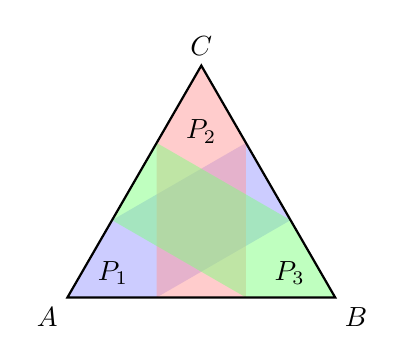
\begin{tikzpicture}[scale=3.4]
  \coordinate (A) at (0,0); \coordinate (B) at (1,0); \coordinate (C) at (0.5,0.866);
  \fill[blue!40,opacity=.5]  (0,0) -- (0.3333,0) -- (0.8333,0.2887)
       -- (0.6667,0.5773) -- (0.1667,0.2887) -- cycle;
  \fill[red!40,opacity=.5]   (0.3333,0) -- (0.6667,0) -- (0.6667,0.5773)
       -- (0.5,0.866) -- (0.3333,0.5773) -- cycle;
  \fill[green!50,opacity=.5] (0.6667,0) -- (1,0) -- (0.8333,0.2887)
       -- (0.3333,0.5773) -- (0.1667,0.2887) -- cycle;
  \draw[thick] (A) -- (B) -- (C) -- cycle;
  \node[below left]  at (A) {$A$};
  \node[below right] at (B) {$B$};
  \node[above]       at (C) {$C$};
  \node at (0.17,0.09)  {$P_1$};
  \node at (0.5,0.62)   {$P_2$};
  \node at (0.83,0.09)  {$P_3$};
\end{tikzpicture}
\caption{The tight median covering of Theorem~\ref{thm:median}:
$I_1=I_2=I_3=[\tfrac13,\tfrac23]$. Each plank $P_i=\{m_i\in[\tfrac13,\tfrac23]\}$
is the central-thirds band of its median; the three traces tile each edge, and
the planks cover $\Delta$ with $\sum\rw=1$.}
\label{fig:median}
\end{figure}
\begin{proof}[Proof of the bound]
Let $\mu$ be the perimeter measure: uniform in the parameter on each of the three
edges, mass $\tfrac13$ each. A direct computation shows each pushforward
$m_{i\#}\mu=\Leb[0,1]$: $\mu$ is a witness measure, certifying
$D(m_1,m_2,m_3)=1$ in the language of Definition~\ref{def:defect}. Indeed for $m_1$: on $AB$, $m_1$ ranges over $[0,\tfrac12]$
with Jacobian $2$ (density $\tfrac13\cdot2$); on $CA$, over $[\tfrac12,1]$ likewise;
on $BC$, over $[0,1]$ with Jacobian $1$ (density $\tfrac13$); the total density is
$1$ on $[0,1]$. Hence $\mu(P_i)=\Leb(I_i)=r_i$,
and $1=\mu(\Delta)\le\sum\mu(P_i)\le\sum r_i$.
\end{proof}
\begin{proof}[Proof of rigidity]
Equality in $1\le\sum\mu(P_i)$ forces the $P_i$ to
partition $\mu$ a.e.; since $\mu$ lives on the edges, \emph{on each edge the three
traces tile $[0,1]$}. We claim there are exactly three such edge-tilings, and only
one covers the interior.

\emph{Three edge-tilings.} On each edge each median is affine, so the three traces
are explicit intervals depending piecewise-linearly on $(l_i,h_i)$ through
$a_i=|I_i\cap[0,\tfrac12]|$ and $b_i=|I_i\cap[\tfrac12,1]|$. Classifying each $I_i$ by
crossing type (contained in $[0,\tfrac12]$, crossing $\tfrac12$, or contained in
$[\tfrac12,1]$) and each edge by the left-to-right order of its traces, the abutting
(tiling) conditions become a finite family of linear systems in $(l_i,h_i)$.

\begin{lemma}\label{lem:three}
The edge-tiling conditions have exactly three solutions with $0\le l_i<h_i\le1$:
$[\tfrac13,\tfrac23]^3$, $[0,\tfrac13]^3$, and $[\tfrac23,1]^3$.
\end{lemma}
This is the case $\tau_i=\tfrac12$ of Proposition~\ref{prop:tilings}, proved in
full in Appendix~\ref{app:tilings} for arbitrary cyclic triples: the symmetries
of the configuration reduce the a priori $27$ crossing patterns to seven
classes, five of which are impossible and two of which lead to cyclic linear
systems with unique solutions. The lemma has also been verified by three
independent exact computer enumerations, archived as ancillary files.

\emph{Interior witness.} The centroid $G$ has $m(G)=(\tfrac12,\tfrac12,\tfrac12)$.
Since $\tfrac12\notin[0,\tfrac13]\cup[\tfrac23,1]$, the tilings $[0,\tfrac13]^3$ and
$[\tfrac23,1]^3$ leave $G$ uncovered; they tile the boundary but are not coverings
of $\Delta$. The tiling $[\tfrac13,\tfrac23]^3$ covers $\Delta$ and has
$\sum r_i=1$. Hence the unique covering with $\sum r_i=1$ is $[\tfrac13,\tfrac23]^3$.
\end{proof}

\section{A dimension-agnostic necessary condition for transport}\label{sec:concur}
The proofs of Theorems~\ref{thm:twodir} and~\ref{thm:median} share one device: a
probability measure whose pushforward under each direction is uniform. Which
direction-tuples admit one?
\begin{proposition}\label{prop:concur}
Let $u_1,\dots,u_{d+1}$ be normalized affine forms on $\Delta^d$ with vertex-value
matrix $V$ invertible. If a probability measure $\mu$ on $\Delta^d$ has
$u_{i\#}\mu=\Leb[0,1]$ for all $i$, then its barycenter $p\in\Delta^d$ satisfies
$Vp=\tfrac12\mathbf 1$; equivalently the mid-level hyperplanes $\{u_i=\tfrac12\}$
concur at $p$, which requires $\mathbf 1^\top V^{-1}\mathbf 1=2$ and
$V^{-1}\mathbf 1\ge0$.
\end{proposition}
\begin{proof}
$\tfrac12=\mathbb E_\mu[u_i]=\sum_j V_{ij}\mathbb E_\mu[x_j]=(Vp)_i$, and
$p\in\Delta^d$ gives $\mathbf 1^\top p=1$, $p\ge0$; substitute $p=\tfrac12V^{-1}\mathbf1$.
\end{proof}
The three medians satisfy this with $p$ the centroid; the three facets do not
($\mathbf 1^\top V^{-1}\mathbf 1=3\ne2$), recovering Gardner's obstruction. The
concurrence family is two-dimensional (parametrized by $p$): a normalized direction
has vertex values $\{0,\tau,1\}$, and $Vp=\tfrac12\mathbf1$ ties each $\tau_i$ to $p$.
The medians are the case $p=$ centroid, forcing $\tau_i=\tfrac12$. Among these, the
explicit perimeter measure singles out the medians:
\begin{proposition}\label{prop:tauhalf}
For a direction $u$ with vertex values $\{0,\tau,1\}$, the perimeter measure $\mu$
(uniform on each edge, mass $\tfrac13$) satisfies $u_\#\mu=\Leb[0,1]$ if and only if
$\tau=\tfrac12$.
\end{proposition}
\begin{proof}
On the three edges $u$ is affine between the pairs $\{0,\tau\},\{\tau,1\},\{0,1\}$,
so $u_\#\mu$ has density $\tfrac1{3\tau}+\tfrac13$ on $[0,\tau]$ and
$\tfrac1{3(1-\tau)}+\tfrac13$ on $[\tau,1]$. Both equal $1$ iff $\tau=\tfrac12$.
\end{proof}
Uniform edge-weights thus single out the medians. Allowing \emph{unequal} edge
masses, however, the construction covers a full two-parameter family:
\begin{theorem}[weighted perimeter]\label{thm:wper}
Let $p=(p_A,p_B,p_C)$ be interior with $\max_j p_j<\tfrac12$, and let
$u_1=(\tau_1,0,1)$, $u_2=(0,1,\tau_2)$, $u_3=(1,\tau_3,0)$ (vertex values at
$A,B,C$) be the cyclic directions concurrent at $p$, i.e.\
$\tau_1=\frac{1/2-p_C}{p_A}$, $\tau_2=\frac{1/2-p_B}{p_C}$,
$\tau_3=\frac{1/2-p_A}{p_B}$. Let $\mu_p$ be uniform on each edge with masses
$w_{AB}=1-2p_C$, $w_{BC}=1-2p_A$, $w_{CA}=1-2p_B$ (summing to $1$). We fix
once and for all the \emph{mass convention}
\[
\alpha:=w_{BC}=1-2p_A,\qquad \beta:=w_{CA}=1-2p_B,\qquad
\gamma:=w_{AB}=1-2p_C:
\]
each Greek letter names the mass of the edge \emph{opposite} the like-named
vertex. This convention is used verbatim in Theorem~\ref{thm:tight} and in
\S\ref{sec:defect}. Then
$u_{i\#}\mu_p=\Leb[0,1]$ for $i=1,2,3$; consequently every covering of $\Delta$ by
planks in these three directions satisfies $\sum\rw\ge1$.
\end{theorem}
\begin{proof}
Each $u_i$ is affine of full range $[0,1]$ on the edge joining its $0$- and
$1$-vertices ($u_1$ on $BC$, $u_2$ on $AB$, $u_3$ on $CA$) and affine of range
$[0,\tau_i]$, resp.\ $[\tau_i,1]$, on the other two. The pushforward of a uniform
edge mass $w_e$ through an affine map of range length $L$ is uniform with density
$w_e/L$. Hence $u_{1\#}\mu_p$ has density $w_{BC}+w_{AB}/\tau_1$ on $[0,\tau_1]$ and
$w_{BC}+w_{CA}/(1-\tau_1)$ on $[\tau_1,1]$, and similarly for $u_2,u_3$: six
equations. Using $p_A+p_B+p_C=1$, each composite term collapses by the identity
$(1-2x)\,p/(\tfrac12-x)=2p$: e.g.\
$w_{AB}/\tau_1=(1-2p_C)p_A/(\tfrac12-p_C)=2p_A$, so
$w_{BC}+w_{AB}/\tau_1=(1-2p_A)+2p_A=1$; likewise
$1-\tau_1=\frac{1/2-p_B}{p_A}$ gives $w_{CA}/(1-\tau_1)=2p_A$. All six densities
equal $1$, so each marginal is $\Leb[0,1]$, and the transport argument of
Theorem~\ref{thm:median} applies verbatim. Finally $\tau_i\in(0,1)$ for all $i$ iff
$\max_jp_j<\tfrac12$ iff all three masses are positive, so every valid cyclic triple
admits $\mu_p$.
\end{proof}
Taking $p$ the centroid recovers Theorem~\ref{thm:median}'s bound ($\tau_i=\tfrac12$,
equal masses). For $p$ off the centroid the directions are tilted non-median
triples; e.g.\ $p=(\tfrac9{20},\tfrac3{10},\tfrac14)$ gives
$\tau=(\tfrac59,\tfrac45,\tfrac16)$ with masses $(\tfrac12,\tfrac1{10},\tfrac25)$.
Theorem~\ref{thm:wper} thus proves the bound of Conjecture~\ref{conj:bang} for a
two-parameter family of direction triples on the triangle, answering the
finite-direction existence question of~\cite{Gardner88} affirmatively for the cyclic
concurrent family. Figure~\ref{fig:wper} shows the running example.

\begin{figure}[ht]
\centering
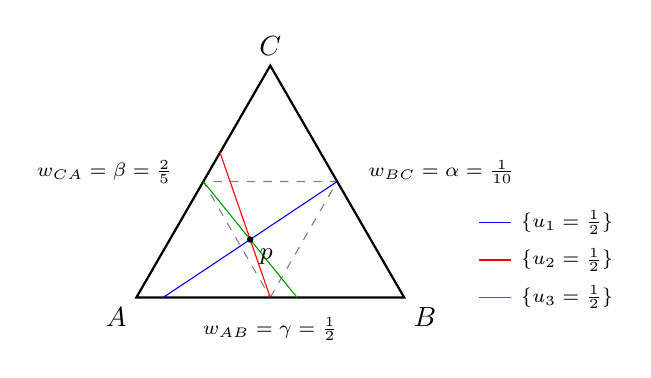
\begin{tikzpicture}[scale=3.4]
  \coordinate (A) at (0,0); \coordinate (B) at (1,0); \coordinate (C) at (0.5,0.866);
  \draw[dashed,gray] (0.5,0) -- (0.75,0.433) -- (0.25,0.433) -- cycle;
  \draw[thick] (A) -- (B) -- (C) -- cycle;
  \draw[blue]  (0.1,0)    -- (0.75,0.433);
  \draw[red]   (0.5,0)    -- (0.3125,0.54125);
  \draw[green!60!black] (0.6,0) -- (0.25,0.433);
  \fill (0.425,0.2165) circle (0.012) node[below right,font=\small] {$p$};
  \node[below left]  at (A) {$A$};
  \node[below right] at (B) {$B$};
  \node[above]       at (C) {$C$};
  \node[below,font=\scriptsize] at (0.5,-0.04) {$w_{AB}=\gamma=\tfrac12$};
  \node[right,font=\scriptsize] at (0.83,0.47) {$w_{BC}=\alpha=\tfrac1{10}$};
  \node[left,font=\scriptsize]  at (0.17,0.47) {$w_{CA}=\beta=\tfrac25$};
  \begin{scope}[shift={(1.28,0.08)}]
    \draw[blue] (0,0.2) -- (0.12,0.2)
      node[right,font=\scriptsize,black] {$\{u_1=\tfrac12\}$};
    \draw[red] (0,0.06) -- (0.12,0.06)
      node[right,font=\scriptsize,black] {$\{u_2=\tfrac12\}$};
    \draw[green!60!black] (0,-0.08) -- (0.12,-0.08)
      node[right,font=\scriptsize,black] {$\{u_3=\tfrac12\}$};
  \end{scope}
\end{tikzpicture}
\caption{The weighted-perimeter witness of Theorem~\ref{thm:wper} at
$p=(\tfrac9{20},\tfrac3{10},\tfrac14)$, i.e.\
$\tau=(\tfrac59,\tfrac45,\tfrac16)$: the three mid-level lines $\{u_i=\tfrac12\}$
concur at $p$, which lies in the open medial triangle (dashed), and $\mu_p$ puts
the indicated masses uniformly on the edges.}
\label{fig:wper}
\end{figure}

Combining necessity (Proposition~\ref{prop:concur}) with the explicit construction
(Theorem~\ref{thm:wper}) yields a \emph{characterization}:
\begin{corollary}\label{cor:iff}
Call a direction triple \emph{cyclic} if its vertex values are
$u_1=(\tau_1,0,1)$, $u_2=(0,1,\tau_2)$, $u_3=(1,\tau_3,0)$ with
$\tau_i\in(0,1)$. A cyclic triple admits a uniform-marginal witness measure if and
only if the three mid-level lines $\{u_i=\tfrac12\}$ concur. In that case the
concurrence point $p$ automatically lies in the open medial triangle
($p_j>0$ and $p_j<\tfrac12$ for all $j$), and the weighted-perimeter measure
$\mu_p$ of Theorem~\ref{thm:wper} is a witness.
\end{corollary}
\begin{proof}
The vertex-value matrix has $\det V=-(1+\tau_1\tau_2\tau_3)\ne0$, so
Proposition~\ref{prop:concur} applies and gives necessity. Conversely, if the lines
concur at $p$ (a point of the affine plane of $\Delta$, so $\sum_jp_j=1$), then $p$
is the unique solution of $Vp=\tfrac12\mathbf1$, which in closed form reads
$2(1+\tau_1\tau_2\tau_3)\,p_A=1-\tau_3(1-\tau_2)$ and cyclically; each right-hand
side is positive for $\tau_i\in(0,1)$, so $p_j>0$, and the identities
$\tfrac12-p_C=\tau_1p_A$, $\tfrac12-p_A=\tau_3p_B$, $\tfrac12-p_B=\tau_2p_C$ give
$p_j<\tfrac12$. Theorem~\ref{thm:wper} then supplies $\mu_p$.
\end{proof}
\begin{remark}
The \emph{anti-cyclic} pattern (all $0$- and $1$-roles exchanged) reduces to the
cyclic one by a reflection of $\Delta$ (a transposition of two vertices), which
maps the medial triangle to itself; Theorem~\ref{thm:wper},
Corollary~\ref{cor:iff} and Theorem~\ref{thm:tight} below hold for it verbatim.
All remaining role assignments are classified by Theorem~\ref{thm:char} below.
\end{remark}

The bound of Theorem~\ref{thm:wper} is in fact \emph{attained} at every member
of the family, and the tight covering is unique --- a two-parameter family of
sharp configurations extending the median rigidity of \S\ref{sec:median}.

The coverage argument below rests on an elementary topological fact, which we
isolate.

\begin{pocketlemma}
Let $H$ be an open convex subset of the plane of $\Delta$ such that
$P:=H\cap\operatorname{int}\Delta\ne\varnothing$ and the \emph{closure}
$\overline P$ of $P$ meets $\partial\Delta$ in a finite set. Then
$H\subseteq\overline\Delta$; in particular $H$ is bounded.
\end{pocketlemma}

\begin{proof}
Suppose $y\in H\setminus\overline\Delta$, and choose a disk $B\subseteq P$. For
$z\in B$ the segment $[z,y]$ lies in $H$ by convexity and joins
$\operatorname{int}\Delta$ to the complement of $\overline\Delta$; let $w(z)$ be
the first point of $\partial\Delta$ on it, starting from $z$. Then
$[z,w(z))\subseteq H\cap\operatorname{int}\Delta$, so
$w(z)\in\overline P\cap\partial\Delta$, a finite set. But for a fixed boundary
point $w$, every $z$ with $w(z)=w$ lies on the line through $y$ and $w$, and
finitely many lines cannot cover the disk $B$ --- a contradiction.
\end{proof}

\begin{theorem}[tightness and rigidity of the cyclic family]\label{thm:tight}
Let $p$ and $u_1,u_2,u_3$ be as in Theorem~\ref{thm:wper}, with the mass
convention fixed there: $\alpha=w_{BC}=1-2p_A$, $\beta=w_{CA}=1-2p_B$,
$\gamma=w_{AB}=1-2p_C$ ($\alpha,\beta,\gamma>0$, $\alpha+\beta+\gamma=1$). Set
$S=\alpha\beta+\beta\gamma+\gamma\alpha$. Then the planks $P_i=\{u_i\in I_i\}$
with
\[
I_1=\Bigl[\tfrac{\alpha\gamma}S,\,1-\tfrac{\alpha\beta}S\Bigr],\qquad
I_2=\Bigl[\tfrac{\beta\gamma}S,\,1-\tfrac{\alpha\gamma}S\Bigr],\qquad
I_3=\Bigl[\tfrac{\alpha\beta}S,\,1-\tfrac{\beta\gamma}S\Bigr]
\]
cover $\Delta$, with $\sum\rw
=\tfrac{\beta\gamma}S+\tfrac{\alpha\beta}S+\tfrac{\alpha\gamma}S=1$. Moreover
this is the unique covering of $\Delta$ with $\sum\rw=1$ by three planks of
positive width, one in each of the directions $u_1,u_2,u_3$. At $p$ the centroid
($\alpha=\beta=\gamma=\tfrac13$) it is $[\tfrac13,\tfrac23]^3$, recovering
Theorem~\ref{thm:median}.
\end{theorem}

The proof rests on three lemmas, stated with the notation of
Theorem~\ref{thm:tight}. Throughout,
$l=(l_1,l_2,l_3)=(\alpha\gamma,\beta\gamma,\alpha\beta)/S$ and
$h=(h_1,h_2,h_3)=\mathbf1-(\alpha\beta,\alpha\gamma,\beta\gamma)/S$ denote the
interval endpoints, so $I_i=[l_i,h_i]$, and
$\tau_1=\frac{\gamma}{1-\alpha}$, $\tau_2=\frac{\beta}{1-\gamma}$,
$\tau_3=\frac{\alpha}{1-\beta}$ from the formulas of Theorem~\ref{thm:wper}. A
direct substitution shows $(l,h)=(\lambda,\rho)$, the first solution of
Proposition~\ref{prop:tilings}; in particular $l_i<\tau_i<h_i$, and the traces
of $P_1,P_2,P_3$ tile all three edges, so $\partial\Delta\subset\bigcup P_i$.

\begin{lemma}[margin identity]\label{lem:margin}
Let $a_1=\alpha(1-\alpha)$, $a_2=\gamma(1-\gamma)$, $a_3=\beta(1-\beta)$ and
$\Lambda=a_1u_1+a_2u_2+a_3u_3$. Then $\Lambda\equiv S$ on the plane of
$\Delta$, $\sum_ia_i=2S$, and
\begin{equation}\label{eq:margin}
\textstyle\sum_i a_il_i=S-\frac{\alpha\beta\gamma}S<S<
S+\frac{\alpha\beta\gamma}S=\sum_i a_ih_i .
\end{equation}
\end{lemma}

\begin{proof}
At the vertices:
$\Lambda(A)=a_1\tau_1+a_3=\alpha\gamma+\beta(\alpha+\gamma)=S$,
$\Lambda(B)=a_2+a_3\tau_3=\gamma(\alpha+\beta)+\alpha\beta=S$,
$\Lambda(C)=a_1+a_2\tau_2=\alpha(\beta+\gamma)+\beta\gamma=S$. An affine
function agreeing at three affinely independent points is constant:
$\Lambda\equiv S$ on the plane of $\Delta$. Moreover
$\sum_ia_i=1-(\alpha^2+\beta^2+\gamma^2)=2S$, and expanding (using
$1-\alpha=\beta+\gamma$ etc.)
\[
\textstyle\sum_i a_il_i
=\frac{\alpha^2\gamma(\beta+\gamma)+\beta\gamma^2(\alpha+\beta)
+\alpha\beta^2(\gamma+\alpha)}{S}
=\frac{(\alpha^2\beta^2+\beta^2\gamma^2+\gamma^2\alpha^2)+\alpha\beta\gamma}{S}
=\frac{S^2-\alpha\beta\gamma}{S},
\]
since $S^2=\sum\alpha^2\beta^2+2\alpha\beta\gamma$; the same expansion gives
$\sum_ia_i(1-h_i)=\frac{S^2-\alpha\beta\gamma}S$, whence
$\sum_ia_ih_i=2S-\frac{S^2-\alpha\beta\gamma}S=S+\frac{\alpha\beta\gamma}S$.
\end{proof}

\begin{lemma}[coverage]\label{lem:coverage}
The planks $P_i=\{u_i\in[l_i,h_i]\}$, $i=1,2,3$, cover $\Delta$.
\end{lemma}

\begin{proof}
Suppose not; the uncovered set $U$ is
relatively open (planks are closed) and misses the tiled boundary
$\partial\Delta$, and it
decomposes as $U=\bigcup_\sigma P_\sigma$ over the eight sign patterns
$\sigma\in\{\mathrm{lo},\mathrm{hi}\}^3$, where $P_\sigma=H_\sigma\cap
\operatorname{int}\Delta$ and $H_\sigma$ is the open convex set
$\{u_i<l_i\ (\sigma_i=\mathrm{lo}),\ u_i>h_i\ (\sigma_i=\mathrm{hi})\}$; write
$c_i$ for the active bound ($l_i$ or $h_i$). We show each $P_\sigma$ is empty.

First, $\overline{P_\sigma}\cap\partial\Delta$ is finite. Indeed, such a point
$x$ satisfies the closed pattern constraints ($u_j(x)\le l_j$ if
$\sigma_j=\mathrm{lo}$, $u_j(x)\ge h_j$ if $\sigma_j=\mathrm{hi}$), and, lying
on the tiled boundary, is covered by some $P_j$, so $u_j(x)\in[l_j,h_j]$;
together these force $u_j(x)=c_j$ for that $j$. Each $u_j$ is affine and
nonconstant on each edge (its two vertex values there are distinct), so
$\{u_j=c_j\}$ meets each edge in at most one point: at most $3\times3=9$ points
in all --- this count includes the vertices of $\Delta$ (each lies on two
edges) and only drops if several of these constraint points coincide. By the
Pocket Lemma applied to $H_\sigma$ (whose intersection
with $\operatorname{int}\Delta$ is $P_\sigma$),
$H_\sigma\subseteq\overline\Delta$ whenever $P_\sigma\ne\varnothing$; in
particular $H_\sigma$ is bounded.

No two of the lines $\ell_i=\{u_i=c_i\}$ are parallel: $u_i\parallel u_j$ would
force $\tau_1(1-\tau_2)=1$, $\tau_2(1-\tau_3)=1$ or $\tau_3(1-\tau_1)=1$,
impossible for $\tau\in(0,1)^3$. If the three lines are concurrent, $H_\sigma$
is an intersection of three open half-planes whose boundaries pass through one
point, hence empty or an unbounded open cone; boundedness gives
$H_\sigma=\varnothing$. Otherwise $H_\sigma$, if nonempty, is the open triangle
with vertices $v_{ij}=\ell_i\cap\ell_j\in\overline{H_\sigma}
\subseteq\overline\Delta$, and each $v_{ij}$ satisfies the closed constraint in
the third index $k$. Since $\Lambda\equiv S$ (Lemma~\ref{lem:margin}),
$u_k(v_{ij})=(S-a_ic_i-a_jc_j)/a_k$, so that constraint reads $S\le\sum_ma_mc_m$
if $\sigma_k=\mathrm{lo}$, and $S\ge\sum_ma_mc_m$ if $\sigma_k=\mathrm{hi}$. For
a \emph{mixed} pattern both directions occur, forcing $S=\sum_ma_mc_m$; but then
$u_k(v_{ij})=c_k$, i.e.\ the three lines concur --- excluded. For
$\sigma=(\mathrm{lo},\mathrm{lo},\mathrm{lo})$ we get $S\le\sum a_il_i$, and for
$\sigma=(\mathrm{hi},\mathrm{hi},\mathrm{hi})$, $S\ge\sum a_ih_i$ --- both
contradict \eqref{eq:margin}. Hence $U=\varnothing$.
\end{proof}

\begin{lemma}[interior witnesses]\label{lem:witness}
Neither $(\,[0,l_i]\,)_i$ nor $(\,[h_i,1]\,)_i$ covers $\Delta$: with
$\delta=\frac{\alpha\beta\gamma}{2S^2}$, the point $x^\ast$ with
$u_i(x^\ast)=l_i+\delta$ for all $i$ and the point $y^\ast$ with
$u_i(y^\ast)=h_i-\delta$ for all $i$ are interior points of $\Delta$ uncovered
by the respective triple.
\end{lemma}

\begin{proof}
The prescription $u_i(x^\ast)=l_i+\delta$ is consistent with
$\Lambda\equiv S$ by \eqref{eq:margin} and $\sum a_i=2S$, and determines a
unique point of the plane since the vertex-value matrix $V$ is invertible. Its
barycentric coordinates are
\[
x^\ast=\tfrac1{2S^2}\Bigl(\alpha\beta(1-\alpha)(1+\alpha-\beta),\;
\beta\gamma(1-\beta)(\alpha+2\beta),\;
\alpha\gamma(\alpha+\beta)(2-2\alpha-\beta)\Bigr),
\]
all positive: $\alpha,\beta,\gamma>0$ handle the leading factors (with
$1-\alpha=\beta+\gamma>0$), while $1+\alpha-\beta>1-\beta>0$, $\alpha+2\beta>0$,
and $2-2\alpha-\beta=\beta+2\gamma>0$ using $\alpha+\beta+\gamma=1$. So
$x^\ast\in\operatorname{int}\Delta$ and
$u_i(x^\ast)>l_i$ for every $i$: $x^\ast$ is uncovered by
$(\,[0,l_i]\,)$. Symmetrically the point $y^\ast$ with
$u_i(y^\ast)=h_i-\delta$, with coordinates
$\frac1{2S^2}\bigl(\alpha\gamma(1-\alpha)(2\alpha+\beta),\,
\alpha\beta(1-\beta)(1+\beta-\alpha),\,
\beta\gamma(\alpha+\beta)(2-\alpha-2\beta)\bigr)$, positive likewise
($2\alpha+\beta>0$, $1+\beta-\alpha>1-\alpha>0$,
$2-\alpha-2\beta=\alpha+2\gamma>0$), is uncovered by
$(\,[h_i,1]\,)$.
\end{proof}

\begin{proof}[Proof of Theorem~\ref{thm:tight}]
\emph{Coverage and value.} Lemma~\ref{lem:coverage} gives the covering;
$\sum\rw=\sum(h_i-l_i)=1$ is the displayed computation in the statement.

\emph{Uniqueness.} Let $(I_i')$ be any covering with all
$r_i'=|I_i'|>0$ and $\sum r_i'=1$. Since $u_{i\#}\mu_p=\Leb[0,1]$
(Theorem~\ref{thm:wper}), $\mu_p(P_i')=r_i'$, and
$1=\mu_p(\Delta)\le\sum\mu_p(P_i')=1$ forces the planks to partition $\mu_p$
a.e.; as $\mu_p$ has positive uniform density on each edge, the traces tile all
three edges. By Proposition~\ref{prop:tilings}, $(I_i')$ is $(\,[\lambda_i,
\rho_i]\,)=(I_i)$, $(\,[0,\lambda_i]\,)$ or $(\,[\rho_i,1]\,)$. The last two do
not cover $\Delta$ by Lemma~\ref{lem:witness}. Hence $(I_i')=(I_i)$.
\end{proof}

\begin{remark}
At the centroid, $\delta=\tfrac16$ and both witnesses degenerate to the point
with $u_i\equiv\tfrac12$ --- the centroid itself, recovering the interior
witness used in the proof of Theorem~\ref{thm:median}. The identities of
Lemma~\ref{lem:margin} and the positivity of the witness coordinates in
Lemma~\ref{lem:witness}, as well as exact coverage checks
at several family points, are verified symbolically in the archived ancillary
script \texttt{cyclic\_family\_tight\_rigidity.py}.
\end{remark}

Finally, the restriction to cyclic role assignments can be removed altogether.
The plank problem is invariant under the \emph{flip} of a normalized direction,
$u\mapsto1-u$, $I\mapsto1-I$ (the planks, their widths, and uniformity of
marginals are unchanged, and each mid-level line is fixed). Call the edge
joining the $0$- and $1$-vertices of a direction its \emph{full edge}. Flips
reduce every role assignment to one of three shapes, and the existence question
is settled in each:

\begin{theorem}[three-direction characterization]\label{thm:char}
Let $u_1,u_2,u_3$ be normalized directions on $\Delta$, pairwise non-parallel.
A probability measure $\mu$ on $\Delta$ with $u_{i\#}\mu=\Leb[0,1]$ for
$i=1,2,3$ exists if and only if the three mid-level lines $\{u_i=\tfrac12\}$
have a common point $p$. In that case $\sum\rw\ge1$ for every covering of
$\Delta$ by planks parallel to these directions, and exactly one of the
following holds:
\begin{itemize}
\item[(a)] the full edges are pairwise distinct: up to flips the triple is
cyclic, $p$ lies in the open medial triangle, and Theorems~\ref{thm:wper}
and~\ref{thm:tight} apply verbatim (explicit witness $\mu_p$; unique tight
covering);
\item[(b)] all three directions have the same full edge $e$: then $p$ is the
midpoint of $e$, the uniform measure on $e$ is a witness, and the bound follows
from covering $e$ alone (the trivial one-dimensional case recorded in
Theorem~\ref{thm:oned}).
\end{itemize}
\end{theorem}

\begin{proof}
\emph{Necessity.} If $\mu$ exists, its barycenter $p\in\Delta$ satisfies
$u_i(p)=\mathbb E_\mu[u_i]=\tfrac12$ for every $i$ (no invertibility of $V$ is
needed), so the mid-lines concur at $p$.

\emph{Classification.} (1) If the three full edges are distinct, flipping each
direction so that its $(0,1)$-pair is oriented cyclically makes the triple
cyclic; by Corollary~\ref{cor:iff}, concurrence then places $p$ in the open
medial triangle and yields $\mu_p$, and Theorem~\ref{thm:tight} the unique
tight covering. (2) Suppose exactly two directions, say $u_i$ and $u_j$, share
their full edge $e$, and let $x_v$ be the barycentric coordinate of the vertex
$v$ opposite $e$. After a flip, $u_i$ and $u_j$ agree on $e$, so
$u_i-u_j=(\tau_i-\tau_j)x_v$ with $\tau_i\ne\tau_j$ (equality would make them
parallel). Hence $\{u_i=\tfrac12\}\cap\{u_j=\tfrac12\}\subset\{x_v=0\}$, the
line through $e$, on which both mid-lines pass only through the midpoint of
$e$; but the third direction is not full on $e$, its values at the endpoints of
$e$ being $\{0,\tau_k\}$ or $\{\tau_k,1\}$, so its value at the midpoint is
$\tfrac{\tau_k}2$ or $\tfrac{1+\tau_k}2$, never $\tfrac12$. Thus the mid-lines
of such a triple \emph{never} concur; consistently, no witness measure exists
($\mathbb E_\mu[u_i]=\mathbb E_\mu[u_j]=\tfrac12$ would force
$\mathbb E_\mu[x_v]=0$, hence $\operatorname{supp}\mu\subset e$, on which $u_k$
is not onto $[0,1]$). This shape contributes to neither side of the
equivalence. (3) If all three directions share the full edge $e$, then after
flips each restricts to $e$ as the identity parameter, so all mid-lines pass
through the midpoint of $e$ (concurrence always holds), and the uniform
probability measure on $e$ has all three pushforwards equal to $\Leb[0,1]$.
For the bound, a covering of $\Delta$ covers $e$, on which the $i$-th plank
traces an interval of length $r_i$; hence $\sum r_i\ge1$.
\end{proof}

\begin{remark}\label{rem:charscope}
Theorem~\ref{thm:char} answers the existence question of~\cite{Gardner88}
completely --- but \emph{only} --- for three directions on the triangle. In
particular, \emph{within the
uniform-marginal witness-measure approach}, the remaining three-direction case
is that of non-concurrent triples, for which no witness measure can exist. This
is a statement about the reach of the method, not a reduction of
Conjecture~\ref{conj:bang} on the triangle (which concerns arbitrarily many
planks in arbitrary directions).
\end{remark}

The trichotomy of Theorem~\ref{thm:char} in one glance:

\begin{center}
\begin{tabular}{@{}llll@{}}
\hline
full-edge pattern & concurrence & witness support & bound mechanism\\
\hline
three distinct edges & iff mid-lines concur & weighted perimeter $\mu_p$
 & transport, $D=1$,\\
(cyclic, mod flips) & (two-parameter family) & on $\partial\Delta$
 & tight and rigid\\[2pt]
exactly two coincide & never & none exists & transport, $D>1$:\\
 & & & $\sum\rw\ge1/D$ only\\[2pt]
all three coincide, edge $e$ & always (midpoint of $e$) & uniform measure
on $e$ & one-dimensional\\
 & & & reduction\\
\hline
\end{tabular}
\end{center}

Rigidity (Theorem~\ref{thm:tight}) concerns the concurrent members of the
cyclic family. The same canonical configuration, however, \emph{covers} for
every cyclic parameter, with an excess that measures non-concurrence exactly.

\begin{theorem}[canonical covering of an arbitrary cyclic triple]
\label{thm:canon}
Let $\tau\in(0,1)^3$ be any cyclic parameter (no concurrence assumed), and
let $\lambda_i,\rho_i$ be as in Proposition~\ref{prop:tilings}. Write
$\Pi=\tau_1\tau_2\tau_3$ and $Q=(1-\tau_1)(1-\tau_2)(1-\tau_3)$. Then the
planks $P_i=\{u_i\in[\lambda_i,\rho_i]\}$ cover $\Delta$, with
\[
\sum_i\rw(P_i)\;=\;1+\frac{(\Pi-Q)^2}{(1+\Pi)(1+Q)} .
\]
The excess vanishes if and only if $\Pi=Q$, which for cyclic triples is
equivalent to concurrence of the mid-lines; in the concurrent case the
configuration is the unique tight covering of Theorem~\ref{thm:tight}.
\end{theorem}

\begin{proof}
Set $g_i=1-\tau_{i+1}(1-\tau_{i+2})\in(0,1)$ (indices mod $3$), so that
$\lambda_i=\tau_ig_i/(1+\Pi)$ and $\rho_i=g_{i+1}/(1+Q)$ in the formulas of
Proposition~\ref{prop:tilings}. The affine dependency of the triple
(Proposition~\ref{prop:wedge}(i)) has the explicit positive form
\[
\sum_ic_iu_i\equiv1,\qquad c_i=\frac{g_i}{1+\Pi}>0 :
\]
at the vertex $A$, $c_1\tau_1+c_3
=\bigl(\tau_1-\tau_1\tau_2+\Pi+1-\tau_1+\tau_1\tau_2\bigr)/(1+\Pi)=1$, and
similarly at $B$ and $C$. Three polynomial identities, each a direct
expansion (they are also verified symbolically in the ancillary files):
\[
(1+\Pi)^2-\sum_i\tau_ig_i^2=g_1g_2g_3,\qquad
\sum_ig_ig_{i+1}-(1+\Pi)(1+Q)=g_1g_2g_3,
\]
\[
(1+\Pi)\sum_ig_i-(1+Q)\sum_i\tau_ig_i-(1+\Pi)(1+Q)=(\Pi-Q)^2 .
\]
The first two give the strict \emph{margins}
\[
\sum_ic_i\lambda_i=1-\frac{g_1g_2g_3}{(1+\Pi)^2}<1,\qquad
\sum_ic_i\rho_i=1+\frac{g_1g_2g_3}{(1+\Pi)(1+Q)}>1,
\]
and the third is the displayed excess formula, since
$\sum\rw=\sum_i\rho_i-\sum_i\lambda_i
=\bigl(\sum g_i\bigr)/(1+Q)-\bigl(\sum\tau_ig_i\bigr)/(1+\Pi)$.

\emph{Coverage.} By Proposition~\ref{prop:tilings} the traces of the $P_i$
tile all three edges, so $\partial\Delta\subset\bigcup P_i$. The proof of
Lemma~\ref{lem:coverage} now applies verbatim with $(a_i,S)$ replaced by
$(c_i,1)$: the boundary-contact count and the Pocket Lemma are unchanged;
mixed sign patterns force their three level lines to concur and are excluded
by boundedness; and the patterns
$(\mathrm{lo},\mathrm{lo},\mathrm{lo})$, $(\mathrm{hi},\mathrm{hi},\mathrm{hi})$
would force $1\le\sum c_i\lambda_i$, resp.\ $1\ge\sum c_i\rho_i$ ---
contradicting the margins.

\emph{The excess and concurrence.} From $c_i=g_i/(1+\Pi)$,
\[
\textstyle\sum_ic_i=\frac{2+\Pi+Q}{1+\Pi},\qquad
1-\tfrac12\sum_ic_i=\frac{\Pi-Q}{2(1+\Pi)},
\]
using $\sum_ig_i=3-\bigl(\sum\tau_i-\sum\tau_i\tau_{i+1}\bigr)=2+\Pi+Q$. So
the concurrence defect of \S\ref{sec:defect} has the closed form
$\delta_c(u_\tau)=|\Pi-Q|\,/\,\bigl(2(2+\Pi+Q)\bigr)$, and $\Pi=Q$ iff
$\delta_c=0$ iff the mid-lines concur --- necessarily inside $\Delta$
(Lemma~\ref{lem:external}, proved independently in \S\ref{sec:defect}) ---
iff $D(u_\tau)=1$. At $\Pi=Q$ the excess vanishes and the configuration is
the tight covering of Theorem~\ref{thm:tight}.
\end{proof}

\begin{remark}\label{rem:canon}
Theorem~\ref{thm:canon} extends the sharp half of Theorem~\ref{thm:tight}
quantitatively beyond the concurrent locus: \emph{every} cyclic triple
carries a canonical non-degenerate covering whose excess over $1$ is exactly
the \emph{concurrence penalty} $(\Pi-Q)^2/\bigl((1+\Pi)(1+Q)\bigr)$. For the
sandwich parameter $\tau=(\tfrac{13}{25},\tfrac12,\tfrac12)$ of
Remark~\ref{rem:sandwich} the excess is $\tfrac1{12656}$. In the language of
Definition~\ref{def:covconst} this certifies only $C_\Delta(u_\tau)\le1$
(which is trivial); its value is structural --- it exhibits the natural
covering family interpolating the rigid tight coverings, and it feeds the
covering-constant program of \S\ref{sec:problems}.
\end{remark}

\smallskip
The concurrence condition is dimension-agnostic: the cyclic medians of $\Delta^d$
($m_i(e_i)=\tfrac12$, $m_i(e_{i+1})=0$, $m_i(e_{i-1})=1$, else $\tfrac12$) have
row-sums $\tfrac{d+1}2$, hence concur at the centroid in every dimension. (A
caution specific to $d=3$: there $m_{i+2}=1-m_i$, so this literal family collapses
to two directions up to flips; this happens exactly when $d+1$ divides $4$.)
Section~\ref{sec:simplex3} constructs witness measures for a non-degenerate
one-parameter family of concurrent quadruples on $\Delta^3$, extending the
transport method beyond the plane; for $d\ge4$ the question is open
(Problem~\ref{prob:suff}).

\section{Duality and exact values for the transport defect}\label{sec:defect}
Theorem~\ref{thm:char} says the transport method certifies the full bound
$\sum\rw\ge1$ exactly when the mid-lines concur. In the language of
\S\ref{sec:measure}:

\begin{corollary}\label{cor:done}
For a pairwise non-parallel triple $u$ on $\Delta$, $D(u)=1$ if and only if the
three mid-level lines concur; otherwise $D(u)>1$.
\end{corollary}
\begin{proof}
Combine Proposition~\ref{prop:defect}(iii) with Theorem~\ref{thm:char}.
\end{proof}

This section quantifies how the method degrades off the concurrent locus, and
develops the tool that governs the question: a strong linear-programming
duality for $D_K$, with explicit certificates on both sides.

\subsection*{The concurrence defect and the moment bound}
The necessary condition of Proposition~\ref{prop:concur} can be made
quantitative. For a family $u=(u_1,\dots,u_n)$ of directions on a convex body
$K$ define the \emph{concurrence defect}
\begin{equation}\label{eq:cdefect}
\delta(u)\;=\;\min_{p\in K}\ \max_{i}\ \bigl|u_i(p)-\tfrac12\bigr|,
\end{equation}
a minimum of a continuous function on a compact set, hence attained; clearly
$\delta(u)=0$ if and only if the mid-level sets $\{u_i=\tfrac12\}$ have a
common point in $K$. Moreover $\delta(u)<\tfrac12$:
at any interior $p$ each $u_i(p)\in(0,1)$, since an affine function on $K$
attaining its minimum $0$ at an interior point would be identically $0$.

\begin{proposition}[moment bound]\label{prop:moment}
For every family $u$ of directions on a convex body $K$,
$D_K(u)\ge\bigl(1-2\delta(u)\bigr)^{-1}$. In particular, for the facet triple
$u=(\lambda_1,\lambda_2,\lambda_3)$ on the triangle one has $\delta=\tfrac16$
and $D\ge\tfrac32$.
\end{proposition}

\begin{proof}
Let $\nu$ be a probability measure on $[0,1]$ with $\nu\le D\Leb$ and
distribution function $F(t)\le\min(1,Dt)$. Its mean is
$\int_0^1(1-F)\ge\int_0^1\max(0,1-Dt)\,dt=\tfrac1{2D}$, and by the mirror
argument the mean lies in $[\tfrac1{2D},\,1-\tfrac1{2D}]$. If $\mu$ is
admissible for $D$ and $p$ is its barycenter, then $p\in K$ and the mean of
$u_{i\#}\mu$ is $u_i(p)$, so
$\delta(u)\le\max_i|u_i(p)-\tfrac12|\le\tfrac12-\tfrac1{2D}$, which rearranges
to the claim. For the facets, $\sum_i\lambda_i(p)=1$ forces some
$\lambda_i(p)\le\tfrac13$, so $\delta\ge\tfrac16$; the centroid attains
$\tfrac16$.
\end{proof}

On the triangle the concurrence defect --- of \emph{any} family, of any size
--- can never exceed the facet value:

\begin{theorem}[centroid bound]\label{thm:centroid}
For every finite family $u_1,\dots,u_n$ of directions on the triangle,
$\delta(u)\le\tfrac16$, witnessed by the centroid $G$; the facet triple attains
$\tfrac16$. Consequently the moment bound never certifies
$D(u)>\tfrac32$ on the triangle, for any number of directions.
\end{theorem}

\begin{proof}
A direction $u$ has vertex values $\{0,s,1\}$ in some order, $s\in[0,1]$, so
$u(G)=\tfrac{0+s+1}3=\tfrac{1+s}3\in[\tfrac13,\tfrac23]$, i.e.\
$|u(G)-\tfrac12|\le\tfrac16$, for \emph{every} direction simultaneously. For
the facet triple $\delta=\tfrac16$ by Proposition~\ref{prop:moment}. (Equality
$|u(G)-\tfrac12|=\tfrac16$ forces $s\in\{0,1\}$, i.e.\ two equal vertex
values, as for facet directions.)
\end{proof}

Among genuine triples, the extremal case is unique:

\begin{proposition}[uniqueness of the extremal triple]\label{prop:deltamax}
A pairwise non-parallel triple on $\Delta$ has $\delta(u)=\tfrac16$ if and
only if it is the facet triple modulo flips $u\mapsto1-u$.
\end{proposition}

\begin{proof}
Flips of facet directions give $\delta=\tfrac16$ by
Proposition~\ref{prop:moment} ($\delta$ is flip-invariant). Conversely,
suppose $\delta(u)=\tfrac16$. Since
$\delta\le\max_i|u_i(G)-\tfrac12|\le\tfrac16$, the centroid is a minimizer
with value exactly $\tfrac16$. Let $B=\{i:|u_i(G)-\tfrac12|=\tfrac16\}$
($\ne\varnothing$); by the equality analysis in
Theorem~\ref{thm:centroid}, each $i\in B$ has $s_i\in\{0,1\}$, i.e.\
$u_i\in\{x_{v},1-x_{v}\}$ for some vertex $v=v(i)$, where $x_v$ denotes the
barycentric coordinate of $v$; in either case the \emph{improving gradient}
at $G$ (the direction of decrease of $|u_i-\tfrac12|$) is
$g_i=\nabla x_{v(i)}$. If some vector $d$ in the plane of $\Delta$ had
$\langle g_i,d\rangle>0$ for all $i\in B$, then for small $t>0$ the interior
points $G+td$ would satisfy $|u_i-\tfrac12|<\tfrac16$ for $i\in B$ (strict
improvement) and for $i\notin B$ (continuity), contradicting
$\delta=\tfrac16$. By Gordan's alternative, $0$ lies in the convex hull of
$\{g_i:i\in B\}$. Now $|B|=1$ is impossible ($g_i\ne0$), and $|B|=2$ would
force $g_i\parallel g_j$, i.e.\ $u_i\parallel u_j$ --- excluded. So $|B|=3$:
all three directions are of the form $x_v$ or $1-x_v$, and pairwise
non-parallelism forces three \emph{distinct} vertices: the facet triple
modulo flips.
\end{proof}

At the facets the moment bound is exact:

\begin{theorem}\label{thm:facetdefect}
For the facet triple, $D(\lambda_1,\lambda_2,\lambda_3)=\tfrac32$. The infimum
is attained by the uniform probability measure on the perimeter of the inscribed
triangle with vertices
\[
P_0=(0,\tfrac13,\tfrac23),\qquad P_1=(\tfrac23,0,\tfrac13),\qquad
P_2=(\tfrac13,\tfrac23,0),
\]
whose three marginals all equal $\tfrac32\cdot\mathbf 1_{[0,2/3]}$.
\end{theorem}

\begin{proof}
The lower bound is Proposition~\ref{prop:moment}. For the upper bound give each
side of the loop mass $\tfrac13$, uniformly in the parameter. The coordinate
$\lambda_1$ is affine on each side, with values $0\to\tfrac23$ on $P_0P_1$
(density $\tfrac12$ on $[0,\tfrac23]$), $\tfrac23\to\tfrac13$ on $P_1P_2$
(density $1$ on $[\tfrac13,\tfrac23]$), and $\tfrac13\to0$ on $P_2P_0$ (density
$1$ on $[0,\tfrac13]$); the total is $\tfrac32$ on $[0,\tfrac23]$. The loop is
invariant under the cyclic rotation of $\Delta$, so the same holds for
$\lambda_2,\lambda_3$.
\end{proof}

\begin{figure}[ht]
\centering
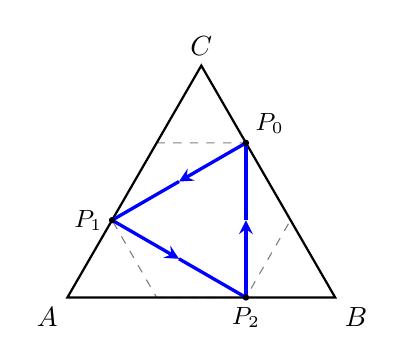
\begin{tikzpicture}[scale=3.4]
  \coordinate (A) at (0,0); \coordinate (B) at (1,0); \coordinate (C) at (0.5,0.866);
  \draw[dashed,gray] (0.3333,0) -- (0.6667,0) -- (0.8333,0.2887)
       -- (0.6667,0.5773) -- (0.3333,0.5773) -- (0.1667,0.2887) -- cycle;
  \draw[thick] (A) -- (B) -- (C) -- cycle;
  \draw[very thick,blue,-stealth] (0.6667,0.5773) -- (0.4167,0.4330);
  \draw[very thick,blue] (0.4167,0.4330) -- (0.1667,0.2887);
  \draw[very thick,blue,-stealth] (0.1667,0.2887) -- (0.4167,0.14435);
  \draw[very thick,blue] (0.4167,0.14435) -- (0.6667,0);
  \draw[very thick,blue,-stealth] (0.6667,0) -- (0.6667,0.28865);
  \draw[very thick,blue] (0.6667,0.28865) -- (0.6667,0.5773);
  \fill (0.6667,0.5773) circle (0.012) node[above right,font=\small] {$P_0$};
  \fill (0.1667,0.2887) circle (0.012) node[left,font=\small] {$P_1$};
  \fill (0.6667,0) circle (0.012) node[below,font=\small] {$P_2$};
  \node[below left]  at (A) {$A$};
  \node[below right] at (B) {$B$};
  \node[above]       at (C) {$C$};
\end{tikzpicture}
\caption{The witness of Theorem~\ref{thm:facetdefect}: the uniform measure on
the inscribed loop $P_0P_1P_2$ (mass $\tfrac13$ per side) has all three
marginals equal to $\tfrac32\cdot\mathbf1_{[0,2/3]}$, so $D=\tfrac32$ for the
facet triple. Dashed: the hexagon $\{\max_i\lambda_i\le\tfrac23\}$, whose
alternate vertices the loop connects.}
\label{fig:loop}
\end{figure}

\begin{remark}\label{rem:complement}
Theorem~\ref{thm:facetdefect} makes precise the complementarity of the two
methods in this paper: for facet directions the tiling argument of
Theorem~\ref{thm:facet} certifies the sharp bound $1$, while the transport
method cannot certify more than $1/D=\tfrac23$ --- and now provably certifies
exactly that. Conversely, for the concurrent cyclic triples the transport bound is
sharp (Theorems~\ref{thm:wper} and~\ref{thm:tight}) where no facet tiling is
available.
\end{remark}

\subsection*{Duality}
$D_K$ is the value of an infinite-dimensional linear program, and it has a
concrete dual. Call a tuple $\psi=(\psi_1,\dots,\psi_n)$ of continuous
functions on $[0,1]$ \emph{admissible} if $\psi_i\ge0$ for all $i$ and
$\sum_i\int_0^1\psi_i(t)\,dt=1$.

\begin{theorem}[minimax duality]\label{thm:duality}
For every convex body $K$ and every family $u_1,\dots,u_n$ of directions on
$K$,
\[
D_K(u)\;=\;\sup_{\psi\ \mathrm{admissible}}\ \ \min_{x\in K}\
\sum_{i=1}^n\psi_i\bigl(u_i(x)\bigr).
\]
Weak duality is elementary and two-sided: every $D$-admissible measure
certifies $D_K(u)\le D$, and every admissible $\psi$ certifies
$D_K(u)\ge\min_{x\in K}\sum_i\psi_i(u_i(x))$. The supremum is unchanged if the
$\psi_i$ range over bounded Borel functions. We do \emph{not} assert that the
supremum is attained in general; it is attained in every exact example of
this paper.
\end{theorem}

\begin{proof}
\emph{Weak duality.} If $\mu$ is $D$-admissible and $\psi$ admissible, then
\[
\min_{x\in K}\sum_i\psi_i(u_i(x))\ \le\
\int_K\sum_i\psi_i(u_i(x))\,d\mu(x)\ =\ \sum_i\int_0^1\psi_i\,d\nu_i\ \le\
D\sum_i\int_0^1\psi_i\,dt\ =\ D,
\]
where $\nu_i:=u_{i\#}\mu$; the middle inequality holds because
$\nu_i\le D\cdot\Leb$ and $\psi_i\ge0$. Since the infimum defining $D_K(u)$ is
attained (Proposition~\ref{prop:defect}(i)), the supremum is at most
$D_K(u)$; the same computation applies verbatim to bounded Borel $\psi_i$, so
enlarging the class cannot raise the supremum past $D_K(u)$.

\emph{The pairing.} For $\mu\in\mathcal P(K)$ and admissible $\psi$ put
$\Phi(\psi,\mu)=\sum_i\int_K\psi_i(u_i(x))\,d\mu(x)$, a bilinear functional.

\emph{Claim 1: for fixed $\mu$,}
$\sup_\psi\Phi(\psi,\mu)=D_{\min}(\mu):=\inf\{D:\nu_i\le D\cdot\Leb\ \forall
i\}\in[1,\infty]$. The inequality $\le$ is the computation above. For $\ge$,
let $1\le D<D_{\min}(\mu)$; then $\nu_i(A)>D|A|$ for some $i$ and some Borel
$A\subseteq[0,1]$. By inner regularity of $\nu_i$ choose a compact $F\subseteq
A$ with $\nu_i(F)>D|A|\ge D|F|$; by outer regularity of Lebesgue measure
choose $U\supseteq F$, relatively open in $[0,1]$, with $D|U|<\nu_i(F)$. By
Urysohn's lemma there is a continuous $g$ with
$\mathbf1_F\le g\le\mathbf1_U$; then $F\ne\varnothing$ (as $\nu_i(F)>0$)
forces $\int_0^1g\,dt>0$, and
\[
\int_0^1 g\,d\nu_i\ \ge\ \nu_i(F)\ >\ D|U|\ \ge\ D\int_0^1g\,dt .
\]
The tuple with $\psi_i=g/\int g\,dt$ and $\psi_j=0$ for $j\ne i$ is
admissible and gives $\Phi>D$. Hence $\sup_\psi\Phi(\psi,\mu)\ge D_{\min}(\mu)$
(for $D<1$ use $\psi_1\equiv1$, which gives $\Phi=1$). By
Definition~\ref{def:defect}, $D_K(u)=\inf_{\mu}D_{\min}(\mu)$.

\emph{Claim 2: for fixed admissible $\psi$,}
$\inf_{\mu\in\mathcal P(K)}\Phi(\psi,\mu)=\min_{x\in
K}\sum_i\psi_i(u_i(x))$: the integrand $x\mapsto\sum_i\psi_i(u_i(x))$ is
continuous on the compact $K$, so the minimum is attained; every
$\mu$-average dominates it, and Dirac measures realize it.

\emph{Minimax.} $\mathcal P(K)$ with the weak-$*$ topology is a compact
convex subset of $C(K)^*$, and the admissible $\psi$ form a convex subset of
the Banach space $C([0,1])^n$. $\Phi$ is bilinear, weak-$*$ continuous in
$\mu$ for fixed $\psi$ (the integrand is continuous on $K$), and sup-norm
continuous in $\psi$ for fixed $\mu$. Sion's minimax theorem~\cite{Sion58}
gives
\[
\inf_{\mu\in\mathcal P(K)}\ \sup_{\psi}\ \Phi(\psi,\mu)\;=\;
\sup_{\psi}\ \inf_{\mu\in\mathcal P(K)}\ \Phi(\psi,\mu).
\]
By Claim~1 the left side is $\inf_\mu D_{\min}(\mu)=D_K(u)$; by Claim~2 the
right side is the asserted supremum.
\end{proof}

\begin{corollary}[certificates]\label{cor:certificates}
Upper bounds for $D_K(u)$ are certified by explicit measures, lower bounds by
explicit admissible $\psi$: verifying a lower bound $B$ requires only the
normalization $\sum_i\int\psi_i=1$ and the pointwise inequality
$\sum_i\psi_i(u_i(x))\ge B$ on $K$ --- no optimization. By
Theorem~\ref{thm:duality} the two sides meet at $D_K(u)$; every exact defect
value in this paper is certified by such a matched pair. (Lower bounds for
$D$ quantify what the transport method \emph{cannot} certify; upper bounds
for $D$ yield covering bounds via Proposition~\ref{prop:defect}(ii).)
\end{corollary}

For the facet triple the dual side is three lines:
$\psi_i(t)=(1-\tfrac32t)_+$ for $i=1,2,3$ is admissible (each integral equals
$\tfrac13$), and pointwise $\psi_i(\lambda_i)\ge1-\tfrac32\lambda_i$, so on
$\Delta$
\[
\textstyle\sum_i\psi_i(\lambda_i)\ \ge\ 3-\tfrac32\sum_i\lambda_i\ =\
\tfrac32 ,
\]
certifying $D\ge\tfrac32$ and matching the loop measure of
Theorem~\ref{thm:facetdefect} exactly. Note where equality lives: the sum
equals $\tfrac32$ precisely on the hexagon
$\{\max_i\lambda_i\le\tfrac23\}$, which carries the inscribed loop, and each
$\psi_i$ vanishes precisely on $[\tfrac23,1]$, where the slack
$\rho_i=\tfrac32\mathbf1_{[2/3,1]}$ of the loop's marginal lives --- the
equality pattern of Proposition~\ref{prop:slack} below in the flesh
(Figure~\ref{fig:dualcert}).

\begin{figure}[ht]
\centering
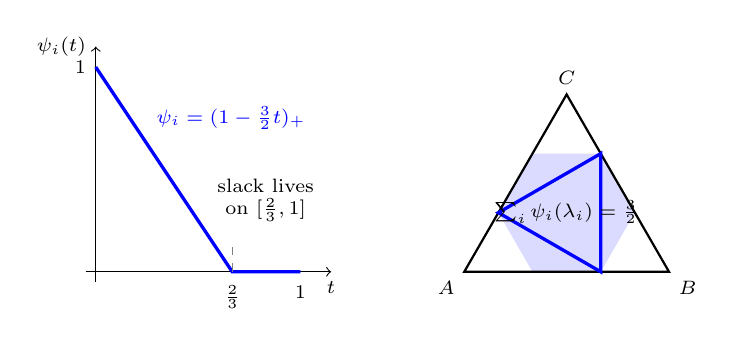
\begin{tikzpicture}[scale=2.6]
  % left panel: the wedge psi
  \draw[->] (-0.05,0) -- (1.15,0) node[below,font=\scriptsize] {$t$};
  \draw[->] (0,-0.05) -- (0,1.1)
    node[left,font=\scriptsize] {$\psi_i(t)$};
  \draw[very thick,blue] (0,1) -- (0.6667,0) -- (1,0);
  \draw[dashed,gray] (0.6667,0) -- (0.6667,0.15);
  \node[below,font=\scriptsize] at (0.6667,-0.02) {$\tfrac23$};
  \node[below,font=\scriptsize] at (1,-0.02) {$1$};
  \node[left,font=\scriptsize] at (0,1) {$1$};
  \node[blue,font=\scriptsize,right] at (0.25,0.75)
    {$\psi_i=(1-\tfrac32t)_+$};
  \node[font=\scriptsize,align=center] at (0.83,0.35)
    {slack lives\\ on $[\tfrac23,1]$};
  % right panel: contact hexagon + loop
  \begin{scope}[shift={(1.8,0)}]
  \coordinate (A) at (0,0); \coordinate (B) at (1,0);
  \coordinate (C) at (0.5,0.866);
  \fill[blue!14] (0.3333,0) -- (0.6667,0) -- (0.8333,0.2887)
       -- (0.6667,0.5773) -- (0.3333,0.5773) -- (0.1667,0.2887) -- cycle;
  \draw[thick] (A) -- (B) -- (C) -- cycle;
  \draw[very thick,blue] (0.6667,0.5773) -- (0.1667,0.2887)
       -- (0.6667,0) -- cycle;
  \node[below left,font=\scriptsize]  at (A) {$A$};
  \node[below right,font=\scriptsize] at (B) {$B$};
  \node[above,font=\scriptsize]       at (C) {$C$};
  \node[font=\scriptsize,align=center] at (0.5,0.29)
    {$\sum_i\psi_i(\lambda_i)=\tfrac32$};
  \end{scope}
\end{tikzpicture}
\caption{The matched primal--dual pair at the facet triple. Left: the dual
certificate $\psi_i(t)=(1-\tfrac32t)_+$ (one wedge per direction, total
integral $1$), which vanishes exactly where the slack of the optimal
marginals lives. Right: the contact set $\{\sum_i\psi_i(\lambda_i)=\tfrac32\}$
is the shaded hexagon $\{\max_i\lambda_i\le\tfrac23\}$, and the optimal
measure --- the inscribed loop of Theorem~\ref{thm:facetdefect} --- is
supported inside it: the equality pattern of
Proposition~\ref{prop:slack}.}
\label{fig:dualcert}
\end{figure}

The moment bound, too, has a dual incarnation: an explicit family of
\emph{wedge} certificates built from the affine dependency of the triple.

\begin{proposition}[wedge certificates]\label{prop:wedge}
Let $u=(u_1,u_2,u_3)$ be pairwise non-parallel directions on $\Delta$.
\begin{itemize}
\item[(i)] There is an affine dependency $\sum_ic_iu_i\equiv c_0$ with
$c=(c_1,c_2,c_3)$, unique up to scale, and all $c_i\ne0$. (The constant may
vanish: $c_0=0$ occurs exactly for the degenerate families all of whose
$u_i$ vanish at a common point of the plane, e.g.\ triples sharing one full
edge; every quantity below is homogeneous of degree $0$ in $(c,c_0)$, so no
normalization is assumed.) Set
$A=\sum_i|c_i|$ and
\[
\kappa_1=c_0-\sum_{c_i<0}c_i,\qquad \kappa_2=\sum_{c_i>0}c_i-c_0 ,
\]
so $\kappa_1+\kappa_2=A$. Then $\kappa_1,\kappa_2>0$, and with
$\kappa=\min(\kappa_1,\kappa_2)$ and $\theta=2\kappa/A\in(0,1]$,
\[
D(u)\ \ge\ \frac{A}{2\kappa}\ =\ \frac1{1-2\delta_c(u)},\qquad
\delta_c(u):=\frac{\bigl|c_0-\tfrac12\sum_ic_i\bigr|}{A},
\]
certified by the admissible wedges
$\psi_i(t)=\frac{2|c_i|}{A\theta^2}\,\bigl(\theta-\varphi_i(t)\bigr)_+$, where
$\varphi_i(t)=t$ for $c_i>0$ and $\varphi_i(t)=1-t$ for $c_i<0$ if
$\kappa=\kappa_1$, and with $t\leftrightarrow1-t$ exchanged if
$\kappa=\kappa_2$.
\item[(ii)] $\delta_c(u)$ is the $\ell^\infty$-distance from the center
$z=(\tfrac12,\tfrac12,\tfrac12)$ to the plane
$\Pi=\{t\in\R^3:\sum_ic_it_i=c_0\}$, which contains the image triangle
$T_u=\{(u_1(x),u_2(x),u_3(x)):x\in\Delta\}$. Hence
$\delta_c(u)\le\delta(u)$: the wedge bound is at most the moment bound.
\item[(iii)] If $\delta_c>0$, the point of $\Pi$ nearest to $z$ in
$\ell^\infty$ is unique, namely $p^\ast$ with
$p^\ast_i=\tfrac12+\epsilon\,\delta_c\operatorname{sign}(c_i)$,
$\epsilon=\operatorname{sign}\bigl(c_0-\tfrac12\sum_ic_i\bigr)$; and
$\delta_c(u)=\delta(u)$ --- i.e.\ the wedge certificate recovers the moment
bound exactly --- if and only if $p^\ast\in T_u$. Theorem~\ref{thm:deltas}
below shows that this criterion is \emph{always} satisfied.
\end{itemize}
\end{proposition}

\begin{proof}
(i) Affine functions on the plane of $\Delta$ form a three-dimensional space,
so $u_1,u_2,u_3,\mathbf1$ are linearly dependent:
$\sum c_iu_i=c_0\mathbf1$ with $(c,c_0)\ne0$, and $c=0$ would force $c_0=0$.
If some $c_i=0$, the relation makes the other two directions parallel ---
excluded; a second, independent relation would eliminate one $u_i$ and make
the remaining two parallel or constant --- also excluded. So $c$ is unique up
to scale with all $c_i\ne0$.

Evaluating the dependency at any $x\in\Delta$,
\[
\kappa_1=c_0-\sum_{c_i<0}c_i
=\sum_{c_i>0}c_iu_i(x)+\sum_{c_i<0}|c_i|\bigl(1-u_i(x)\bigr)\ \ge\ 0,
\]
a \emph{constant} nonnegative combination; if it vanished, each summand would
vanish for every $x$, making some $u_i$ constant ($\equiv0$ or $\equiv1$),
contradicting ontoness. So $\kappa_1>0$, and symmetrically $\kappa_2>0$;
$\kappa_1+\kappa_2=A$ is immediate, whence $\theta=2\kappa/A\le1$.

Say $\kappa=\kappa_1$ (else exchange $t\leftrightarrow1-t$ throughout, which
replaces the telescoped constant below by $\kappa_2$). Since
$\int_0^1(\theta-\varphi_i(t))_+\,dt=\theta^2/2$ for either orientation of
$\varphi_i$, the stated $\psi$ is admissible:
$\sum_i\int\psi_i=\frac{2}{A\theta^2}\cdot A\cdot\frac{\theta^2}2=1$. Pointwise
$(\theta-\varphi)_+\ge\theta-\varphi$ and, by the display above,
$\sum_i|c_i|\varphi_i(u_i(x))=\kappa_1$ for every $x$; hence
\[
\sum_i\psi_i(u_i(x))\ \ge\ \frac{2}{A\theta^2}\Bigl(A\theta-
\sum_i|c_i|\varphi_i(u_i(x))\Bigr)=\frac{2(A\theta-\kappa_1)}{A\theta^2}
=\frac{A}{2\kappa_1}
\]
for $\theta=2\kappa_1/A$. Weak duality (Theorem~\ref{thm:duality}) gives
$D(u)\ge A/(2\kappa)$. Finally $c_0-\tfrac12\sum c_i=\kappa_1-\tfrac A2
=\tfrac A2-\kappa_2$, so $|c_0-\tfrac12\sum c_i|=\tfrac A2-\kappa$ and
$1-2\delta_c=2\kappa/A$.

(ii) The $\ell^\infty$-distance from a point $z$ to the plane
$\{\langle c,t\rangle=c_0\}$ is $|\langle c,z\rangle-c_0|/\|c\|_1$ (dual
norms), which at the center is $\delta_c$. $T_u\subset\Pi$ by the dependency,
and $\delta(u)=\min_{t\in T_u}\|t-z\|_\infty\ge\operatorname{dist}_\infty
(z,\Pi)=\delta_c$.

(iii) For $t\in\Pi$ with $\|t-z\|_\infty=\delta_c$:
$|\langle c,t-z\rangle|=|c_0-\langle c,z\rangle|=\delta_cA$ while
$|\langle c,t-z\rangle|\le\|c\|_1\|t-z\|_\infty=\delta_cA$, with equality only
if $(t-z)_i=\epsilon\,\delta_c\operatorname{sign}(c_i)$ for all $i$ (all
$c_i\ne0$): the nearest point is the single $p^\ast$. Then
$\delta(u)=\delta_c$ iff some point of $T_u$ realizes the plane distance iff
$p^\ast\in T_u$.
\end{proof}

The two defects in fact always coincide. The key is a counting lemma: a
level set of a \emph{common} value can only be shared by few directions at a
point outside the triangle. (At the level $\tfrac12$ this says mid-level
lines of a genuine triple cannot concur outside $\Delta$.)

\begin{lemma}[counting lemma]\label{lem:external}
Let $q$ be a point of the plane of $\Delta$ with $q\notin\Delta$ (some
barycentric coordinate negative; $\sum_jq_j=1$), and let $a\in(0,1)$. Then at
most \emph{two} pairwise non-parallel directions take the value $a$ at $q$.
Consequently: if the three mid-level lines $\{u_i=\tfrac12\}$ of a pairwise
non-parallel triple have a common point $q$, then $q\in\Delta$; and
$\delta_c(u)=0\iff\delta(u)=0\iff D(u)=1$.
\end{lemma}

\begin{proof}
The flip $u\mapsto1-u$ bijects directions with value $a$ at $q$ onto
directions with value $1-a$ at $q$ and preserves parallelism, so we may
assume $a\le\tfrac12$. A direction with value $0$ at vertex $j_0$, $1$ at
vertex $j_1$ and $s\in[0,1]$ at the remaining vertex $j_s$ takes at $q$ the
value $q_{j_1}+s\,q_{j_s}$.

\emph{Case $a=\tfrac12$.} The value condition reads
$q_{j_1}+s\,q_{j_s}=\tfrac12$; since $q_{j_1}+q_{j_s}=1-q_{j_0}$, a solution
$s\in[0,1]$ exists iff $\tfrac12$ lies weakly between $q_{j_1}$ and
$1-q_{j_0}$, iff $(q_{j_0}-\tfrac12)(q_{j_1}-\tfrac12)\ge0$. The ordered
patterns $(j_0,j_1)$ and $(j_1,j_0)$ produce flipped, hence parallel,
directions, so the count is at most the number of \emph{unordered} pairs
$\{j,k\}$ with $(q_j-\tfrac12)(q_k-\tfrac12)\ge0$. All three pairs qualify
only when all $q_j\le\tfrac12$ (all $\ge\tfrac12$ contradicts $\sum q_j=1$),
and then $q_j=1-q_k-q_l\ge0$ for each $j$: $q\in\Delta$, excluded. So the
count is at most $2$.

\emph{Case $a<\tfrac12$.} Write $r_j=q_j-a$ and $r'_j=q_j-(1-a)$, so
$r_j-r'_j=1-2a>0$. First, $q_{j_s}=0$ is impossible for a solvable pattern:
it would force $q_{j_1}=a$ and $q_{j_0}=1-a$, making all coordinates
nonnegative --- but $q\notin\Delta$. So each solvable pattern has the unique
$s=(a-q_{j_1})/q_{j_s}$, and $s\in[0,1]$ iff $a$ lies weakly between
$q_{j_1}$ and $1-q_{j_0}$, iff $r_{j_1}r'_{j_0}\ge0$.

\emph{Parallelism and collisions.} Two directions are parallel iff one is
the flip of the other; the flip of a solution takes value $1-a\ne a$ at $q$,
so distinct solutions are never parallel. A solution with $s\in(0,1)$ has
three distinct vertex values, so its pattern is determined by the direction:
distinct \emph{strict} patterns give distinct directions. The boundary cases
collide: $s=0$ (iff $r_{j_1}=0$) gives the coordinate direction $x_{j_1}$
from \emph{both} patterns with that $j_1$; $s=1$ (iff $r'_{j_0}=0$) gives
$1-x_{j_0}$ from both patterns with that $j_0$. Hence the number $N$ of
distinct pairwise non-parallel directions with value $a$ at $q$ is
\[
N=\#\{\text{solvable patterns with strict signs}\}
+\#\{j:r_j=0\}+\#\{j:r'_j=0\},
\]
the two boundary counts contributing one direction each ($x_j$, resp.\
$1-x_j$; these are pairwise non-parallel for distinct indices, and
$r_j=r'_j=0$ is impossible).

\emph{Counting under externality.} Fix $m$ with $q_m<0$; then $r_m,r'_m<0$
strictly. Let $\{j,k\}$ be the other two indices, so $q_j+q_k=1-q_m>1$. A
pattern $(j_0,j_1)$ is strict iff ($r'_{j_0}>0$ and $r_{j_1}>0$) or
($r'_{j_0}<0$ and $r_{j_1}<0$). Three cases.

(1) \emph{$r_j,r_k\le0$:} then $q_j+q_k\le2a<1$, impossible.

(2) \emph{Exactly one positive, say $r_j>0\ge r_k$:} then
$q_j=1-q_m-q_k>1-a$, so $r'_j>0$ strictly, and
$r'_k=r_k-(1-2a)<0$ strictly. Positive-side strict patterns need
$r_{j_1}>0$ with $j_1\ne j_0=j$: none. Negative-side strict patterns have
$j_0,j_1\in\{k,m\}$: if $r_k<0$, the two patterns $(k,m),(m,k)$ and no
boundary terms; if $r_k=0$, the single pattern $(k,m)$ plus the boundary
direction $x_k$. Either way $N=2$.

(3) \emph{$r_j,r_k>0$:} sub-classify by the signs of $(r'_j,r'_k)$. Both
$>0$: strict patterns $(j,k),(k,j)$ only (a negative-side pattern would need
$j_0=j_1=m$); $N=2$. Signs $(+,-)$: strict patterns $(j,k)$ and $(k,m)$;
$N=2$. Signs $(+,0)$: strict $(j,k)$, boundary $1-x_k$; $N=2$. Both $<0$:
strict $(j,m),(k,m)$; $N=2$. Signs $(0,-)$: strict $(k,m)$, boundary
$1-x_j$; $N=2$. Signs $(0,0)$: no strict patterns, boundaries
$1-x_j,1-x_k$; $N=2$.

In every feasible case $N\le2$, proving the counting statement.

\emph{Consequences.} If the three mid-lines concur at $q$, then three
pairwise non-parallel directions take the value $\tfrac12$ at $q$, so
$q\in\Delta$. If $\delta_c=0$, the center lies on $\Pi$
(Proposition~\ref{prop:wedge}(ii)); the mid-lines of $u_1,u_2$ meet at a
single point $q$, and $c_0=\sum_ic_iu_i(q)=\tfrac12(c_1+c_2)+c_3u_3(q)$
together with $c_0=\tfrac12\sum c_i$ gives $u_3(q)=\tfrac12$ ($c_3\ne0$): the
mid-lines concur at $q\in\Delta$, so $\delta(u)=0$ and $D(u)=1$
(Corollary~\ref{cor:done}). The converses are trivial.
\end{proof}

\begin{theorem}[the two defects coincide]\label{thm:deltas}
For every pairwise non-parallel triple $u$ on $\Delta$,
\[
\delta(u)\;=\;\delta_c(u)\;=\;
\frac{\bigl|c_0-\tfrac12\sum_ic_i\bigr|}{\sum_i|c_i|}\,.
\]
Equivalently, the $\ell^\infty$-projection $p^\ast$ of the center onto $\Pi$
always lies in the image triangle $T_u$, and the single-knot wedge
certificates of Proposition~\ref{prop:wedge} always attain the moment bound.
In particular $\delta$ is an explicit rational function of the vertex data;
for cyclic triples, $\delta(u_\tau)=|\Pi-Q|/\bigl(2(2+\Pi+Q)\bigr)$
(Theorem~\ref{thm:canon}).
\end{theorem}

\begin{proof}
By Proposition~\ref{prop:wedge}(ii) $\delta\ge\delta_c$, with equality iff
$p^\ast\in T_u$ (part (iii)); the case $\delta_c=0$ is
Lemma~\ref{lem:external}. Assume $\delta_c>0$ and, for contradiction,
$p^\ast\notin T_u$.

\emph{Flip normalization.} The flip $u_i\mapsto1-u_i$ replaces
$(c_i,c_0)\mapsto(-c_i,c_0-c_i)$, leaves $\delta$, $\delta_c$ invariant
(both $c_0-\tfrac12\sum c$ and $\sum|c|$ are unchanged), and conjugates
$T_u$ and $p^\ast$ by the reflection $t_i\mapsto1-t_i$ of the $i$-th
coordinate. Flipping every $i$ with $c_i<0$, we may assume all $c_i>0$;
then $p^\ast=(a,a,a)$ with
$a=\tfrac12+\epsilon\delta_c\in(0,1)$ (Proposition~\ref{prop:wedge}(iii),
$\delta_c<\tfrac12$).

\emph{Pulling back.} The evaluation map $E(x)=(u_1(x),u_2(x),u_3(x))$ is an
affine bijection from the plane of $\Delta$ onto $\Pi$: it is injective
because $u_1,u_2$ are non-parallel, hence affine coordinates, and its image
is a $2$-plane contained in $\Pi$, hence equal to it. Let
$q=E^{-1}(p^\ast)$: a point of the plane with $u_i(q)=a$ for $i=1,2,3$, and
$p^\ast\notin T_u=E(\Delta)$ means $q\notin\Delta$.

\emph{Conclusion.} The three directions $u_1,u_2,u_3$ are pairwise
non-parallel and all take the value $a\in(0,1)$ at $q\notin\Delta$ ---
contradicting Lemma~\ref{lem:external}. Hence $p^\ast\in T_u$ and
$\delta=\delta_c$.
\end{proof}

\begin{remark}\label{rem:wedgemoment}
Theorem~\ref{thm:deltas} collapses the a priori hierarchy: for every
pairwise non-parallel triple,
\[
\frac1{1-2\delta_c(u)}\ =\ \frac1{1-2\delta(u)}\ \le\ D(u):
\]
the moment bound \emph{is} the value of the best single-knot wedge pair, in
closed form. The remaining inequality is strict in general: explicit
multi-knot certificates beat the moment bound at explicit triples
(Remark~\ref{rem:sandwich}), and by Theorem~\ref{thm:duality} richer $\psi$
are the \emph{only} possible source of better lower bounds. For the facet
triple both defects equal $\tfrac16$ and the wedge certificate ($c=(1,1,1)$,
$c_0=1$, $\theta=\tfrac23$) is precisely the facet $\psi$ displayed above;
for the sandwich triple both equal $\tfrac1{450}$.
\end{remark}

\begin{proposition}[equality pattern]\label{prop:slack}
Let $\mu$ be a $D$-admissible measure and $\psi$ an admissible tuple with
$\min_{x\in K}\sum_i\psi_i(u_i(x))=D$. Then $D=D_K(u)$, both are optimal,
and:
\begin{itemize}
\item[(i)] $\mu$ is supported on the \emph{contact set}
$C_\psi=\bigl\{x\in K:\sum_i\psi_i(u_i(x))=D\bigr\}$;
\item[(ii)] for each $i$, $\int\psi_i\,d\rho_i=0$, where
$\rho_i=D\cdot\Leb-u_{i\#}\mu\ge0$ is the slack (i.e.\ $\psi_i$ vanishes
$\rho_i$-a.e.).
\end{itemize}
Conversely, if a $D$-admissible $\mu$ and an admissible
$\psi$ satisfy (ii) and $\mu$ is supported on the set where
$\sum_i\psi_i\circ u_i$ attains its minimum over $K$, then
$D=D_K(u)$ and both are optimal.
\end{proposition}

\begin{proof}
The weak-duality chain
\[
D=\min_{x\in K}\sum_i\psi_i(u_i(x))\ \le\ \int_K\sum_i\psi_i(u_i)\,d\mu
\ =\ D\sum_i\int\psi_i\,dt-\sum_i\int\psi_i\,d\rho_i\ \le\ D
\]
collapses to equalities. Equality on the left forces the continuous integrand
$\sum_i\psi_i\circ u_i$ (which is $\ge D$ everywhere) to equal $D$ on
$\operatorname{supp}\mu$: (i). Equality on the right forces
$\sum_i\int\psi_i\,d\rho_i=0$ with nonnegative summands: (ii). Optimality:
$\mu$ certifies $D_K(u)\le D$ and $\psi$ certifies $D_K(u)\ge D$. For the
converse, let $c=\min_{x\in K}\sum_i\psi_i(u_i(x))$; the support condition
gives $\int\sum_i\psi_i(u_i)\,d\mu=c$, while (ii) gives
$\int\sum_i\psi_i(u_i)\,d\mu=D\sum_i\int\psi_i=D$; so $c=D$ and the first
part applies.
\end{proof}

\begin{remark}[skeleton measures and where the optimum lives]
\label{rem:skeleton}
Let $D_\partial(u)$ denote the infimum of Definition~\ref{def:defect}
restricted to measures supported on $\partial\Delta$; always
$D(u)\le D_\partial(u)$. On the concurrent locus
$D_\partial=D=1$: the witness $\mu_p$ of Theorem~\ref{thm:wper} lives on
$\partial\Delta$. At the facet triple, by contrast, $D_\partial=+\infty$:
any probability measure on $\partial\Delta$ gives positive mass to some
closed edge, on which the opposite barycentric coordinate vanishes
identically, so some marginal has an atom at $0$ and no level $D$ is
feasible --- the optimum abandons the boundary entirely (the loop of
Theorem~\ref{thm:facetdefect} is interior). For cyclic triples every
direction is nonconstant on every edge, $D_\partial(u)$ is finite, and
restricted to piecewise-uniform edge densities it is a finite linear program
with rational data: its value is a certified upper bound
(Corollary~\ref{cor:certificates}). By Proposition~\ref{prop:slack},
$D_\partial(u)=D(u)$ exactly when some optimal measure is supported on
$\partial\Delta$ --- equivalently, when the contact set of some dual
optimizer supports one. Whether that holds anywhere off the concurrent locus
is open (Remark~\ref{rem:sandwich}, Problem~\ref{prob:defect}).
\end{remark}

\subsection*{Stability near the concurrent locus}
Near the concurrent locus the defect is small, with an explicit modulus; this
gives bounds beyond the general constant of~\cite{BY26} on open sets of
non-concurrent triples, for coverings in the corresponding direction families
(see Remark~\ref{rem:beyond}).

\begin{theorem}\label{thm:defectstab}
Let $\tau^*\in(0,1)^3$ be a concurrent cyclic parameter with edge masses
$(\alpha,\beta,\gamma)$ as in Theorem~\ref{thm:wper}, and let
$m=\min_i\min(\tau_i^*,1-\tau_i^*)$. If $\tau\in(0,1)^3$ is a cyclic parameter
with $\varepsilon:=\max_i|\tau_i-\tau_i^*|<m$, then
\[
D(u_\tau)\ \le\ 1+\frac{\varepsilon}{m(m-\varepsilon)},
\qquad\text{hence}\qquad
\sum\rw\ \ge\ \frac{m(m-\varepsilon)}{m(m-\varepsilon)+\varepsilon}
\]
for every covering of $\Delta$ by planks parallel to the directions of $\tau$.
\end{theorem}

\begin{proof}
Keep the \emph{frozen} weights: let $\mu$ be the measure with masses
$(\gamma,\alpha,\beta)$ on the edges $(AB,BC,CA)$ --- the mass convention of
Theorem~\ref{thm:wper} --- uniform in the parameter, and
push it forward by the \emph{perturbed} directions. For $u_1$ (vertex values
$(\tau_1,0,1)$) the marginal density is $\alpha+\gamma/\tau_1$ on $[0,\tau_1]$
and $\alpha+\beta/(1-\tau_1)$ on $[\tau_1,1]$; at $\tau_1^*$ both equal $1$ by
the choice of weights in Theorem~\ref{thm:wper}. Subtracting,
\[
\Bigl(\alpha+\frac{\gamma}{\tau_1}\Bigr)-1
=\frac{\gamma\,(\tau_1^*-\tau_1)}{\tau_1\tau_1^*},\qquad
\Bigl(\alpha+\frac{\beta}{1-\tau_1}\Bigr)-1
=\frac{\beta\,(\tau_1-\tau_1^*)}{(1-\tau_1)(1-\tau_1^*)},
\]
and since $\gamma,\beta\le1$, $\tau_1^*\ge m$, $1-\tau_1^*\ge m$ and
$\tau_1,1-\tau_1\ge m-\varepsilon$, both deviations are at most
$\varepsilon/(m(m-\varepsilon))$ in absolute value; the same computation applies
to $u_2,u_3$. Hence $u_{i\#}\mu\le(1+\varepsilon/(m(m-\varepsilon)))\Leb$ for
all $i$, and Proposition~\ref{prop:defect}(ii) gives the covering bound: for
$x=\varepsilon/(m(m-\varepsilon))$ the exact reciprocal is
$1/(1+x)=m(m-\varepsilon)/\bigl(m(m-\varepsilon)+\varepsilon\bigr)$.
\end{proof}

Stability runs in both directions: a small defect forces near-concurrence,
by our own moment bound.

\begin{proposition}[inverse stability]\label{prop:invstab}
If $D(u)\le1+\eta$ for a family $u$ on a convex body $K$, then
$\delta(u)\le\dfrac{\eta}{2(1+\eta)}$.
\end{proposition}

\begin{proof}
By Proposition~\ref{prop:moment}, $(1-2\delta(u))^{-1}\le D(u)\le1+\eta$, so
$1-2\delta(u)\ge(1+\eta)^{-1}$, which rearranges to the claim.
\end{proof}

With Theorem~\ref{thm:defectstab} in one direction and
Proposition~\ref{prop:invstab} in the other, $D(u)-1$ is a two-sided
quantitative measure of non-concurrence on the cyclic family: it vanishes
exactly on the concurrent locus (Corollary~\ref{cor:done}) and is comparable
to the concurrence defect on both sides.

\begin{corollary}\label{cor:beyond}
Every covering of $\Delta$ by planks parallel to the directions of a cyclic
parameter $\tau$ with $\max_i|\tau_i-\tfrac12|\le\tfrac1{60}$ satisfies
\[
\sum\rw\ \ge\ \tfrac{29}{31}\ >\ 4\sqrt3-6 .
\]
\end{corollary}

\begin{proof}
Apply Theorem~\ref{thm:defectstab} with $\tau^*=(\tfrac12,\tfrac12,\tfrac12)$
(the medians, concurrent with $\alpha=\beta=\gamma=\tfrac13$), $m=\tfrac12$,
$\varepsilon=\tfrac1{60}$: here $m(m-\varepsilon)=\tfrac{29}{120}$ and
$m(m-\varepsilon)+\varepsilon=\tfrac{31}{120}$, so
$D\le\tfrac{31}{29}$ and $\sum\rw\ge\tfrac{29}{31}$. The comparison
$\tfrac{29}{31}>4\sqrt3-6$ is $29+6\cdot31=215>124\sqrt3$, i.e.\
$215^2=46225>46128=48\cdot31^2$.
\end{proof}

The medians play no special role: Theorem~\ref{thm:defectstab} certifies an
explicit open neighbourhood of the \emph{whole} concurrent family on which
the transport bound exceeds the numerical value of $4\sqrt3-6$.

\begin{corollary}[a certified neighbourhood of the concurrent locus]
\label{cor:region}
Set $k=\tfrac{2\sqrt3-3}6$, so that $1+k=\tfrac1{4\sqrt3-6}$. Let $\tau^*$ be
any concurrent cyclic parameter and $m=\min_i\min(\tau_i^*,1-\tau_i^*)$. Then
every cyclic parameter $\tau$ with
\[
\max_i|\tau_i-\tau_i^*|\ <\ \frac{km^2}{1+km}
\]
satisfies $D(u_\tau)<\tfrac1{4\sqrt3-6}$, hence $\sum\rw>4\sqrt3-6$ for every
covering of $\Delta$ by planks parallel to the directions of $\tau$. The
union of these boxes over the two-parameter concurrent family is an explicit
open set of triples --- almost all of them non-concurrent --- with a
transport bound past the constant of~\cite{BY26}, subject to the caveat of
Remark~\ref{rem:beyond}. It is the region certified by the upper bound of
Theorem~\ref{thm:defectstab}, not a description of the full sublevel set
$\{D<\tfrac1{4\sqrt3-6}\}$, whose exact extent we do not know.
\end{corollary}

\begin{proof}
Put $\varepsilon=\max_i|\tau_i-\tau_i^*|$. From
$\varepsilon<\frac{km^2}{1+km}<m$ (the latter since $km<1+km$), the
hypothesis of Theorem~\ref{thm:defectstab} holds, and
$\varepsilon(1+km)<km^2$ rearranges to
$\frac\varepsilon{m(m-\varepsilon)}<k$, so
$D(u_\tau)\le1+\frac\varepsilon{m(m-\varepsilon)}<1+k=\tfrac1{4\sqrt3-6}$;
Proposition~\ref{prop:defect}(ii) converts this into the covering bound. For
$\tau^*$ the medians ($m=\tfrac12$) the box radius is
$\frac{k}{4+2k}>\tfrac1{60}$ (equivalent to $58k>4$, i.e.\ to
$10092>9801$), so Corollary~\ref{cor:beyond} is strictly inside this region.
\end{proof}

\begin{remark}\label{rem:beyond}
The set of triples covered by Corollary~\ref{cor:beyond} is a full-dimensional
neighbourhood in the three-parameter space of cyclic triples, and the concurrent
ones form a codimension-one subset of it: the corollary is a bound strictly
inside non-concurrent territory, where by Theorem~\ref{thm:char} no witness
measure exists and $\sum\rw\ge1$ remains open. We stress the honest comparison:
the bound $4\sqrt3-6$ of~\cite{BY26} is uniform over \emph{all} direction
triples, while ours improves on it only on this neighbourhood; far from the
concurrent locus the moment bound (Proposition~\ref{prop:moment}) shows the
transport method degrades irreparably --- at the facets down to $\tfrac23$.
\end{remark}

\begin{remark}[the moment bound is not exact: three certificates]
\label{rem:sandwich}
The two sides of Theorem~\ref{thm:duality} sandwich $D(u)$ between finite,
exactly verifiable computations: skeleton linear programs give certified
\emph{upper} bounds (Remark~\ref{rem:skeleton}), explicit admissible $\psi$
give certified \emph{lower} bounds --- and any feasible $\psi$, however
found, is a rigorous bound. Piecewise-linear $\psi$ with several knots do
strictly beat the moment bound. Three archival certificates, each verified
from scratch by exact rational arithmetic in the ancillary file
\texttt{dual\_certificates.py}:
\begin{center}
\begin{tabular}{@{}lll@{}}
\hline
triple & moment bound $\tfrac1{1-2\delta}$ & certified dual bound\\
\hline
tilted facets, $\varepsilon=\tfrac1{10}$ & $\tfrac{15}{11}\approx1.3636$
 & $D\ge\tfrac{18}{13}\approx1.3846$\\
two shared full edges, $(\tfrac23,\tfrac56,\tfrac1{12})$
 & $\tfrac{153}{142}\approx1.0775$ & $D\ge\tfrac{32}{29}\approx1.1034$\\
cyclic sandwich, $\tau=(\tfrac{13}{25},\tfrac12,\tfrac12)$
 & $\tfrac{225}{224}$ & $D>\tfrac{225}{224}$ (strict)\\
\hline
\end{tabular}
\end{center}
(Here \emph{tilted facets} is the cyclic-symmetric triple with vertex values
$(1,\varepsilon,0)$, $(0,1,\varepsilon)$, $(\varepsilon,0,1)$, and the
second row is a triple with two shared full edges.) In particular
$D(u)=(1-2\delta(u))^{-1}$ is \emph{false} in general, although it holds at
the facet triple in every dimension (Theorem~\ref{thm:facetd}) and trivially
on the concurrent locus. For the sandwich parameter the certificates now
give the strict two-sided bracket
\[
\tfrac{225}{224}\ <\ D(u_\tau)\ \le\ \tfrac{112}{111},
\]
the upper bound being the optimal piecewise-uniform edge-skeleton measure;
whether the upper bound is exact --- equivalently, by
Proposition~\ref{prop:slack} and Remark~\ref{rem:skeleton}, whether some
optimal measure is skeletal here --- remains open.
\end{remark}

The defect also behaves continuously enough to be mapped. Two statements,
one general and one along a degeneration path:

\begin{proposition}[lower semicontinuity]\label{prop:lsc}
On families of $n$ directions with fixed combinatorics, parametrized by
their vertex values, $D_K$ is lower semicontinuous.
\end{proposition}

\begin{proof}
For fixed admissible $\psi$, the map
$u\mapsto\min_{x\in K}\sum_i\psi_i(u_i(x))$ is continuous (the integrand is
jointly continuous and $K$ is compact). By Theorem~\ref{thm:duality},
$D_K$ is the supremum of these functions, hence lower semicontinuous.
\end{proof}

\begin{remark}[a parallel degeneration path]\label{rem:parallelpath}
Upper semicontinuity can fail to be obvious where the family degenerates ---
e.g.\ as two directions become parallel, where Theorem~\ref{thm:twodir}
(via~\cite{Gardner88}) makes the limiting pair have $D=1$. Along the
explicit path $u(\varepsilon)$ with vertex values $(0,1,\tfrac13)$,
$(0,1,\tfrac13+\varepsilon)$, $(\tfrac12,0,1)$ (two shared full edges;
$u_2\to u_1$ as $\varepsilon\downarrow0$), exact two-sided bounds hold for
all $\varepsilon\in(0,\tfrac23)$:
\[
1+\frac{3\varepsilon}{2(3\varepsilon+4)}\ \le\ D\bigl(u(\varepsilon)\bigr)
\ \le\ 1+\tfrac34\varepsilon ,
\]
the lower bound from Theorem~\ref{thm:deltas} (the dependency is
$c=\bigl(\frac{\varepsilon+4/3}\varepsilon,\,-\frac4{3\varepsilon},\,2\bigr)$,
$c_0=1$), the upper from the explicit skeleton measure with edge masses
$\bigl(\frac{1+3\varepsilon}4,\frac{2-3\varepsilon}4,\frac14\bigr)$, whose
marginal densities are all $\le1+\tfrac34\varepsilon$ (a symbolic
verification is archived). So $D\to1$ linearly at this parallel
degeneration: no jump.
\end{remark}

\begin{figure}[ht]
\centering
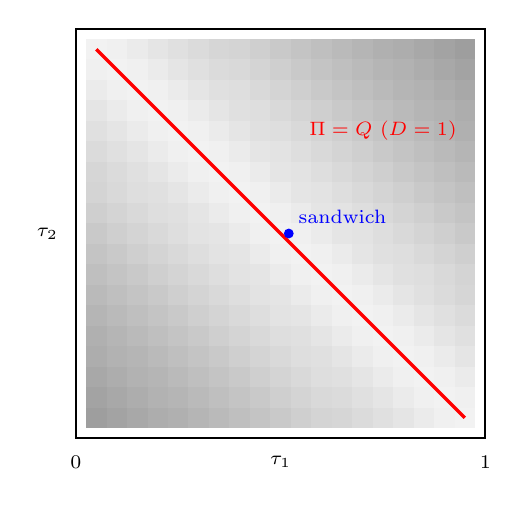
\begin{tikzpicture}[scale=5.2]
\fill[black!38] (0.0250,0.0250) rectangle +(0.0500,0.0500);
\fill[black!36] (0.0250,0.0750) rectangle +(0.0500,0.0500);
\fill[black!34] (0.0250,0.1250) rectangle +(0.0500,0.0500);
\fill[black!32] (0.0250,0.1750) rectangle +(0.0500,0.0500);
\fill[black!31] (0.0250,0.2250) rectangle +(0.0500,0.0500);
\fill[black!29] (0.0250,0.2750) rectangle +(0.0500,0.0500);
\fill[black!27] (0.0250,0.3250) rectangle +(0.0500,0.0500);
\fill[black!25] (0.0250,0.3750) rectangle +(0.0500,0.0500);
\fill[black!23] (0.0250,0.4250) rectangle +(0.0500,0.0500);
\fill[black!21] (0.0250,0.4750) rectangle +(0.0500,0.0500);
\fill[black!19] (0.0250,0.5250) rectangle +(0.0500,0.0500);
\fill[black!17] (0.0250,0.5750) rectangle +(0.0500,0.0500);
\fill[black!16] (0.0250,0.6250) rectangle +(0.0500,0.0500);
\fill[black!14] (0.0250,0.6750) rectangle +(0.0500,0.0500);
\fill[black!12] (0.0250,0.7250) rectangle +(0.0500,0.0500);
\fill[black!10] (0.0250,0.7750) rectangle +(0.0500,0.0500);
\fill[black!8] (0.0250,0.8250) rectangle +(0.0500,0.0500);
\fill[black!6] (0.0250,0.8750) rectangle +(0.0500,0.0500);
\fill[black!5] (0.0250,0.9250) rectangle +(0.0500,0.0500);
\fill[black!36] (0.0750,0.0250) rectangle +(0.0500,0.0500);
\fill[black!34] (0.0750,0.0750) rectangle +(0.0500,0.0500);
\fill[black!32] (0.0750,0.1250) rectangle +(0.0500,0.0500);
\fill[black!30] (0.0750,0.1750) rectangle +(0.0500,0.0500);
\fill[black!29] (0.0750,0.2250) rectangle +(0.0500,0.0500);
\fill[black!27] (0.0750,0.2750) rectangle +(0.0500,0.0500);
\fill[black!25] (0.0750,0.3250) rectangle +(0.0500,0.0500);
\fill[black!23] (0.0750,0.3750) rectangle +(0.0500,0.0500);
\fill[black!21] (0.0750,0.4250) rectangle +(0.0500,0.0500);
\fill[black!19] (0.0750,0.4750) rectangle +(0.0500,0.0500);
\fill[black!17] (0.0750,0.5250) rectangle +(0.0500,0.0500);
\fill[black!15] (0.0750,0.5750) rectangle +(0.0500,0.0500);
\fill[black!14] (0.0750,0.6250) rectangle +(0.0500,0.0500);
\fill[black!12] (0.0750,0.6750) rectangle +(0.0500,0.0500);
\fill[black!10] (0.0750,0.7250) rectangle +(0.0500,0.0500);
\fill[black!8] (0.0750,0.7750) rectangle +(0.0500,0.0500);
\fill[black!6] (0.0750,0.8250) rectangle +(0.0500,0.0500);
\fill[black!5] (0.0750,0.8750) rectangle +(0.0500,0.0500);
\fill[black!6] (0.0750,0.9250) rectangle +(0.0500,0.0500);
\fill[black!34] (0.1250,0.0250) rectangle +(0.0500,0.0500);
\fill[black!32] (0.1250,0.0750) rectangle +(0.0500,0.0500);
\fill[black!30] (0.1250,0.1250) rectangle +(0.0500,0.0500);
\fill[black!29] (0.1250,0.1750) rectangle +(0.0500,0.0500);
\fill[black!27] (0.1250,0.2250) rectangle +(0.0500,0.0500);
\fill[black!25] (0.1250,0.2750) rectangle +(0.0500,0.0500);
\fill[black!23] (0.1250,0.3250) rectangle +(0.0500,0.0500);
\fill[black!21] (0.1250,0.3750) rectangle +(0.0500,0.0500);
\fill[black!19] (0.1250,0.4250) rectangle +(0.0500,0.0500);
\fill[black!17] (0.1250,0.4750) rectangle +(0.0500,0.0500);
\fill[black!15] (0.1250,0.5250) rectangle +(0.0500,0.0500);
\fill[black!13] (0.1250,0.5750) rectangle +(0.0500,0.0500);
\fill[black!12] (0.1250,0.6250) rectangle +(0.0500,0.0500);
\fill[black!10] (0.1250,0.6750) rectangle +(0.0500,0.0500);
\fill[black!8] (0.1250,0.7250) rectangle +(0.0500,0.0500);
\fill[black!6] (0.1250,0.7750) rectangle +(0.0500,0.0500);
\fill[black!5] (0.1250,0.8250) rectangle +(0.0500,0.0500);
\fill[black!6] (0.1250,0.8750) rectangle +(0.0500,0.0500);
\fill[black!8] (0.1250,0.9250) rectangle +(0.0500,0.0500);
\fill[black!32] (0.1750,0.0250) rectangle +(0.0500,0.0500);
\fill[black!30] (0.1750,0.0750) rectangle +(0.0500,0.0500);
\fill[black!29] (0.1750,0.1250) rectangle +(0.0500,0.0500);
\fill[black!27] (0.1750,0.1750) rectangle +(0.0500,0.0500);
\fill[black!25] (0.1750,0.2250) rectangle +(0.0500,0.0500);
\fill[black!23] (0.1750,0.2750) rectangle +(0.0500,0.0500);
\fill[black!21] (0.1750,0.3250) rectangle +(0.0500,0.0500);
\fill[black!19] (0.1750,0.3750) rectangle +(0.0500,0.0500);
\fill[black!17] (0.1750,0.4250) rectangle +(0.0500,0.0500);
\fill[black!15] (0.1750,0.4750) rectangle +(0.0500,0.0500);
\fill[black!13] (0.1750,0.5250) rectangle +(0.0500,0.0500);
\fill[black!12] (0.1750,0.5750) rectangle +(0.0500,0.0500);
\fill[black!10] (0.1750,0.6250) rectangle +(0.0500,0.0500);
\fill[black!8] (0.1750,0.6750) rectangle +(0.0500,0.0500);
\fill[black!6] (0.1750,0.7250) rectangle +(0.0500,0.0500);
\fill[black!5] (0.1750,0.7750) rectangle +(0.0500,0.0500);
\fill[black!6] (0.1750,0.8250) rectangle +(0.0500,0.0500);
\fill[black!8] (0.1750,0.8750) rectangle +(0.0500,0.0500);
\fill[black!10] (0.1750,0.9250) rectangle +(0.0500,0.0500);
\fill[black!31] (0.2250,0.0250) rectangle +(0.0500,0.0500);
\fill[black!29] (0.2250,0.0750) rectangle +(0.0500,0.0500);
\fill[black!27] (0.2250,0.1250) rectangle +(0.0500,0.0500);
\fill[black!25] (0.2250,0.1750) rectangle +(0.0500,0.0500);
\fill[black!23] (0.2250,0.2250) rectangle +(0.0500,0.0500);
\fill[black!21] (0.2250,0.2750) rectangle +(0.0500,0.0500);
\fill[black!19] (0.2250,0.3250) rectangle +(0.0500,0.0500);
\fill[black!17] (0.2250,0.3750) rectangle +(0.0500,0.0500);
\fill[black!15] (0.2250,0.4250) rectangle +(0.0500,0.0500);
\fill[black!13] (0.2250,0.4750) rectangle +(0.0500,0.0500);
\fill[black!12] (0.2250,0.5250) rectangle +(0.0500,0.0500);
\fill[black!10] (0.2250,0.5750) rectangle +(0.0500,0.0500);
\fill[black!8] (0.2250,0.6250) rectangle +(0.0500,0.0500);
\fill[black!6] (0.2250,0.6750) rectangle +(0.0500,0.0500);
\fill[black!5] (0.2250,0.7250) rectangle +(0.0500,0.0500);
\fill[black!6] (0.2250,0.7750) rectangle +(0.0500,0.0500);
\fill[black!8] (0.2250,0.8250) rectangle +(0.0500,0.0500);
\fill[black!10] (0.2250,0.8750) rectangle +(0.0500,0.0500);
\fill[black!12] (0.2250,0.9250) rectangle +(0.0500,0.0500);
\fill[black!29] (0.2750,0.0250) rectangle +(0.0500,0.0500);
\fill[black!27] (0.2750,0.0750) rectangle +(0.0500,0.0500);
\fill[black!25] (0.2750,0.1250) rectangle +(0.0500,0.0500);
\fill[black!23] (0.2750,0.1750) rectangle +(0.0500,0.0500);
\fill[black!21] (0.2750,0.2250) rectangle +(0.0500,0.0500);
\fill[black!19] (0.2750,0.2750) rectangle +(0.0500,0.0500);
\fill[black!17] (0.2750,0.3250) rectangle +(0.0500,0.0500);
\fill[black!15] (0.2750,0.3750) rectangle +(0.0500,0.0500);
\fill[black!13] (0.2750,0.4250) rectangle +(0.0500,0.0500);
\fill[black!11] (0.2750,0.4750) rectangle +(0.0500,0.0500);
\fill[black!10] (0.2750,0.5250) rectangle +(0.0500,0.0500);
\fill[black!8] (0.2750,0.5750) rectangle +(0.0500,0.0500);
\fill[black!6] (0.2750,0.6250) rectangle +(0.0500,0.0500);
\fill[black!5] (0.2750,0.6750) rectangle +(0.0500,0.0500);
\fill[black!6] (0.2750,0.7250) rectangle +(0.0500,0.0500);
\fill[black!8] (0.2750,0.7750) rectangle +(0.0500,0.0500);
\fill[black!10] (0.2750,0.8250) rectangle +(0.0500,0.0500);
\fill[black!12] (0.2750,0.8750) rectangle +(0.0500,0.0500);
\fill[black!14] (0.2750,0.9250) rectangle +(0.0500,0.0500);
\fill[black!27] (0.3250,0.0250) rectangle +(0.0500,0.0500);
\fill[black!25] (0.3250,0.0750) rectangle +(0.0500,0.0500);
\fill[black!23] (0.3250,0.1250) rectangle +(0.0500,0.0500);
\fill[black!21] (0.3250,0.1750) rectangle +(0.0500,0.0500);
\fill[black!19] (0.3250,0.2250) rectangle +(0.0500,0.0500);
\fill[black!17] (0.3250,0.2750) rectangle +(0.0500,0.0500);
\fill[black!15] (0.3250,0.3250) rectangle +(0.0500,0.0500);
\fill[black!13] (0.3250,0.3750) rectangle +(0.0500,0.0500);
\fill[black!11] (0.3250,0.4250) rectangle +(0.0500,0.0500);
\fill[black!10] (0.3250,0.4750) rectangle +(0.0500,0.0500);
\fill[black!8] (0.3250,0.5250) rectangle +(0.0500,0.0500);
\fill[black!6] (0.3250,0.5750) rectangle +(0.0500,0.0500);
\fill[black!5] (0.3250,0.6250) rectangle +(0.0500,0.0500);
\fill[black!6] (0.3250,0.6750) rectangle +(0.0500,0.0500);
\fill[black!8] (0.3250,0.7250) rectangle +(0.0500,0.0500);
\fill[black!10] (0.3250,0.7750) rectangle +(0.0500,0.0500);
\fill[black!12] (0.3250,0.8250) rectangle +(0.0500,0.0500);
\fill[black!14] (0.3250,0.8750) rectangle +(0.0500,0.0500);
\fill[black!16] (0.3250,0.9250) rectangle +(0.0500,0.0500);
\fill[black!25] (0.3750,0.0250) rectangle +(0.0500,0.0500);
\fill[black!23] (0.3750,0.0750) rectangle +(0.0500,0.0500);
\fill[black!21] (0.3750,0.1250) rectangle +(0.0500,0.0500);
\fill[black!19] (0.3750,0.1750) rectangle +(0.0500,0.0500);
\fill[black!17] (0.3750,0.2250) rectangle +(0.0500,0.0500);
\fill[black!15] (0.3750,0.2750) rectangle +(0.0500,0.0500);
\fill[black!13] (0.3750,0.3250) rectangle +(0.0500,0.0500);
\fill[black!11] (0.3750,0.3750) rectangle +(0.0500,0.0500);
\fill[black!10] (0.3750,0.4250) rectangle +(0.0500,0.0500);
\fill[black!8] (0.3750,0.4750) rectangle +(0.0500,0.0500);
\fill[black!6] (0.3750,0.5250) rectangle +(0.0500,0.0500);
\fill[black!5] (0.3750,0.5750) rectangle +(0.0500,0.0500);
\fill[black!6] (0.3750,0.6250) rectangle +(0.0500,0.0500);
\fill[black!8] (0.3750,0.6750) rectangle +(0.0500,0.0500);
\fill[black!10] (0.3750,0.7250) rectangle +(0.0500,0.0500);
\fill[black!12] (0.3750,0.7750) rectangle +(0.0500,0.0500);
\fill[black!13] (0.3750,0.8250) rectangle +(0.0500,0.0500);
\fill[black!15] (0.3750,0.8750) rectangle +(0.0500,0.0500);
\fill[black!17] (0.3750,0.9250) rectangle +(0.0500,0.0500);
\fill[black!23] (0.4250,0.0250) rectangle +(0.0500,0.0500);
\fill[black!21] (0.4250,0.0750) rectangle +(0.0500,0.0500);
\fill[black!19] (0.4250,0.1250) rectangle +(0.0500,0.0500);
\fill[black!17] (0.4250,0.1750) rectangle +(0.0500,0.0500);
\fill[black!15] (0.4250,0.2250) rectangle +(0.0500,0.0500);
\fill[black!13] (0.4250,0.2750) rectangle +(0.0500,0.0500);
\fill[black!11] (0.4250,0.3250) rectangle +(0.0500,0.0500);
\fill[black!10] (0.4250,0.3750) rectangle +(0.0500,0.0500);
\fill[black!8] (0.4250,0.4250) rectangle +(0.0500,0.0500);
\fill[black!6] (0.4250,0.4750) rectangle +(0.0500,0.0500);
\fill[black!5] (0.4250,0.5250) rectangle +(0.0500,0.0500);
\fill[black!6] (0.4250,0.5750) rectangle +(0.0500,0.0500);
\fill[black!8] (0.4250,0.6250) rectangle +(0.0500,0.0500);
\fill[black!10] (0.4250,0.6750) rectangle +(0.0500,0.0500);
\fill[black!12] (0.4250,0.7250) rectangle +(0.0500,0.0500);
\fill[black!13] (0.4250,0.7750) rectangle +(0.0500,0.0500);
\fill[black!15] (0.4250,0.8250) rectangle +(0.0500,0.0500);
\fill[black!17] (0.4250,0.8750) rectangle +(0.0500,0.0500);
\fill[black!19] (0.4250,0.9250) rectangle +(0.0500,0.0500);
\fill[black!21] (0.4750,0.0250) rectangle +(0.0500,0.0500);
\fill[black!19] (0.4750,0.0750) rectangle +(0.0500,0.0500);
\fill[black!17] (0.4750,0.1250) rectangle +(0.0500,0.0500);
\fill[black!15] (0.4750,0.1750) rectangle +(0.0500,0.0500);
\fill[black!13] (0.4750,0.2250) rectangle +(0.0500,0.0500);
\fill[black!11] (0.4750,0.2750) rectangle +(0.0500,0.0500);
\fill[black!10] (0.4750,0.3250) rectangle +(0.0500,0.0500);
\fill[black!8] (0.4750,0.3750) rectangle +(0.0500,0.0500);
\fill[black!6] (0.4750,0.4250) rectangle +(0.0500,0.0500);
\fill[black!5] (0.4750,0.4750) rectangle +(0.0500,0.0500);
\fill[black!6] (0.4750,0.5250) rectangle +(0.0500,0.0500);
\fill[black!8] (0.4750,0.5750) rectangle +(0.0500,0.0500);
\fill[black!10] (0.4750,0.6250) rectangle +(0.0500,0.0500);
\fill[black!11] (0.4750,0.6750) rectangle +(0.0500,0.0500);
\fill[black!13] (0.4750,0.7250) rectangle +(0.0500,0.0500);
\fill[black!15] (0.4750,0.7750) rectangle +(0.0500,0.0500);
\fill[black!17] (0.4750,0.8250) rectangle +(0.0500,0.0500);
\fill[black!19] (0.4750,0.8750) rectangle +(0.0500,0.0500);
\fill[black!21] (0.4750,0.9250) rectangle +(0.0500,0.0500);
\fill[black!19] (0.5250,0.0250) rectangle +(0.0500,0.0500);
\fill[black!17] (0.5250,0.0750) rectangle +(0.0500,0.0500);
\fill[black!15] (0.5250,0.1250) rectangle +(0.0500,0.0500);
\fill[black!13] (0.5250,0.1750) rectangle +(0.0500,0.0500);
\fill[black!12] (0.5250,0.2250) rectangle +(0.0500,0.0500);
\fill[black!10] (0.5250,0.2750) rectangle +(0.0500,0.0500);
\fill[black!8] (0.5250,0.3250) rectangle +(0.0500,0.0500);
\fill[black!6] (0.5250,0.3750) rectangle +(0.0500,0.0500);
\fill[black!5] (0.5250,0.4250) rectangle +(0.0500,0.0500);
\fill[black!6] (0.5250,0.4750) rectangle +(0.0500,0.0500);
\fill[black!8] (0.5250,0.5250) rectangle +(0.0500,0.0500);
\fill[black!10] (0.5250,0.5750) rectangle +(0.0500,0.0500);
\fill[black!11] (0.5250,0.6250) rectangle +(0.0500,0.0500);
\fill[black!13] (0.5250,0.6750) rectangle +(0.0500,0.0500);
\fill[black!15] (0.5250,0.7250) rectangle +(0.0500,0.0500);
\fill[black!17] (0.5250,0.7750) rectangle +(0.0500,0.0500);
\fill[black!19] (0.5250,0.8250) rectangle +(0.0500,0.0500);
\fill[black!21] (0.5250,0.8750) rectangle +(0.0500,0.0500);
\fill[black!23] (0.5250,0.9250) rectangle +(0.0500,0.0500);
\fill[black!17] (0.5750,0.0250) rectangle +(0.0500,0.0500);
\fill[black!15] (0.5750,0.0750) rectangle +(0.0500,0.0500);
\fill[black!13] (0.5750,0.1250) rectangle +(0.0500,0.0500);
\fill[black!12] (0.5750,0.1750) rectangle +(0.0500,0.0500);
\fill[black!10] (0.5750,0.2250) rectangle +(0.0500,0.0500);
\fill[black!8] (0.5750,0.2750) rectangle +(0.0500,0.0500);
\fill[black!6] (0.5750,0.3250) rectangle +(0.0500,0.0500);
\fill[black!5] (0.5750,0.3750) rectangle +(0.0500,0.0500);
\fill[black!6] (0.5750,0.4250) rectangle +(0.0500,0.0500);
\fill[black!8] (0.5750,0.4750) rectangle +(0.0500,0.0500);
\fill[black!10] (0.5750,0.5250) rectangle +(0.0500,0.0500);
\fill[black!11] (0.5750,0.5750) rectangle +(0.0500,0.0500);
\fill[black!13] (0.5750,0.6250) rectangle +(0.0500,0.0500);
\fill[black!15] (0.5750,0.6750) rectangle +(0.0500,0.0500);
\fill[black!17] (0.5750,0.7250) rectangle +(0.0500,0.0500);
\fill[black!19] (0.5750,0.7750) rectangle +(0.0500,0.0500);
\fill[black!21] (0.5750,0.8250) rectangle +(0.0500,0.0500);
\fill[black!23] (0.5750,0.8750) rectangle +(0.0500,0.0500);
\fill[black!25] (0.5750,0.9250) rectangle +(0.0500,0.0500);
\fill[black!16] (0.6250,0.0250) rectangle +(0.0500,0.0500);
\fill[black!14] (0.6250,0.0750) rectangle +(0.0500,0.0500);
\fill[black!12] (0.6250,0.1250) rectangle +(0.0500,0.0500);
\fill[black!10] (0.6250,0.1750) rectangle +(0.0500,0.0500);
\fill[black!8] (0.6250,0.2250) rectangle +(0.0500,0.0500);
\fill[black!6] (0.6250,0.2750) rectangle +(0.0500,0.0500);
\fill[black!5] (0.6250,0.3250) rectangle +(0.0500,0.0500);
\fill[black!6] (0.6250,0.3750) rectangle +(0.0500,0.0500);
\fill[black!8] (0.6250,0.4250) rectangle +(0.0500,0.0500);
\fill[black!10] (0.6250,0.4750) rectangle +(0.0500,0.0500);
\fill[black!11] (0.6250,0.5250) rectangle +(0.0500,0.0500);
\fill[black!13] (0.6250,0.5750) rectangle +(0.0500,0.0500);
\fill[black!15] (0.6250,0.6250) rectangle +(0.0500,0.0500);
\fill[black!17] (0.6250,0.6750) rectangle +(0.0500,0.0500);
\fill[black!19] (0.6250,0.7250) rectangle +(0.0500,0.0500);
\fill[black!21] (0.6250,0.7750) rectangle +(0.0500,0.0500);
\fill[black!23] (0.6250,0.8250) rectangle +(0.0500,0.0500);
\fill[black!25] (0.6250,0.8750) rectangle +(0.0500,0.0500);
\fill[black!27] (0.6250,0.9250) rectangle +(0.0500,0.0500);
\fill[black!14] (0.6750,0.0250) rectangle +(0.0500,0.0500);
\fill[black!12] (0.6750,0.0750) rectangle +(0.0500,0.0500);
\fill[black!10] (0.6750,0.1250) rectangle +(0.0500,0.0500);
\fill[black!8] (0.6750,0.1750) rectangle +(0.0500,0.0500);
\fill[black!6] (0.6750,0.2250) rectangle +(0.0500,0.0500);
\fill[black!5] (0.6750,0.2750) rectangle +(0.0500,0.0500);
\fill[black!6] (0.6750,0.3250) rectangle +(0.0500,0.0500);
\fill[black!8] (0.6750,0.3750) rectangle +(0.0500,0.0500);
\fill[black!10] (0.6750,0.4250) rectangle +(0.0500,0.0500);
\fill[black!11] (0.6750,0.4750) rectangle +(0.0500,0.0500);
\fill[black!13] (0.6750,0.5250) rectangle +(0.0500,0.0500);
\fill[black!15] (0.6750,0.5750) rectangle +(0.0500,0.0500);
\fill[black!17] (0.6750,0.6250) rectangle +(0.0500,0.0500);
\fill[black!19] (0.6750,0.6750) rectangle +(0.0500,0.0500);
\fill[black!21] (0.6750,0.7250) rectangle +(0.0500,0.0500);
\fill[black!23] (0.6750,0.7750) rectangle +(0.0500,0.0500);
\fill[black!25] (0.6750,0.8250) rectangle +(0.0500,0.0500);
\fill[black!27] (0.6750,0.8750) rectangle +(0.0500,0.0500);
\fill[black!29] (0.6750,0.9250) rectangle +(0.0500,0.0500);
\fill[black!12] (0.7250,0.0250) rectangle +(0.0500,0.0500);
\fill[black!10] (0.7250,0.0750) rectangle +(0.0500,0.0500);
\fill[black!8] (0.7250,0.1250) rectangle +(0.0500,0.0500);
\fill[black!6] (0.7250,0.1750) rectangle +(0.0500,0.0500);
\fill[black!5] (0.7250,0.2250) rectangle +(0.0500,0.0500);
\fill[black!6] (0.7250,0.2750) rectangle +(0.0500,0.0500);
\fill[black!8] (0.7250,0.3250) rectangle +(0.0500,0.0500);
\fill[black!10] (0.7250,0.3750) rectangle +(0.0500,0.0500);
\fill[black!12] (0.7250,0.4250) rectangle +(0.0500,0.0500);
\fill[black!13] (0.7250,0.4750) rectangle +(0.0500,0.0500);
\fill[black!15] (0.7250,0.5250) rectangle +(0.0500,0.0500);
\fill[black!17] (0.7250,0.5750) rectangle +(0.0500,0.0500);
\fill[black!19] (0.7250,0.6250) rectangle +(0.0500,0.0500);
\fill[black!21] (0.7250,0.6750) rectangle +(0.0500,0.0500);
\fill[black!23] (0.7250,0.7250) rectangle +(0.0500,0.0500);
\fill[black!25] (0.7250,0.7750) rectangle +(0.0500,0.0500);
\fill[black!27] (0.7250,0.8250) rectangle +(0.0500,0.0500);
\fill[black!29] (0.7250,0.8750) rectangle +(0.0500,0.0500);
\fill[black!31] (0.7250,0.9250) rectangle +(0.0500,0.0500);
\fill[black!10] (0.7750,0.0250) rectangle +(0.0500,0.0500);
\fill[black!8] (0.7750,0.0750) rectangle +(0.0500,0.0500);
\fill[black!6] (0.7750,0.1250) rectangle +(0.0500,0.0500);
\fill[black!5] (0.7750,0.1750) rectangle +(0.0500,0.0500);
\fill[black!6] (0.7750,0.2250) rectangle +(0.0500,0.0500);
\fill[black!8] (0.7750,0.2750) rectangle +(0.0500,0.0500);
\fill[black!10] (0.7750,0.3250) rectangle +(0.0500,0.0500);
\fill[black!12] (0.7750,0.3750) rectangle +(0.0500,0.0500);
\fill[black!13] (0.7750,0.4250) rectangle +(0.0500,0.0500);
\fill[black!15] (0.7750,0.4750) rectangle +(0.0500,0.0500);
\fill[black!17] (0.7750,0.5250) rectangle +(0.0500,0.0500);
\fill[black!19] (0.7750,0.5750) rectangle +(0.0500,0.0500);
\fill[black!21] (0.7750,0.6250) rectangle +(0.0500,0.0500);
\fill[black!23] (0.7750,0.6750) rectangle +(0.0500,0.0500);
\fill[black!25] (0.7750,0.7250) rectangle +(0.0500,0.0500);
\fill[black!27] (0.7750,0.7750) rectangle +(0.0500,0.0500);
\fill[black!29] (0.7750,0.8250) rectangle +(0.0500,0.0500);
\fill[black!30] (0.7750,0.8750) rectangle +(0.0500,0.0500);
\fill[black!32] (0.7750,0.9250) rectangle +(0.0500,0.0500);
\fill[black!8] (0.8250,0.0250) rectangle +(0.0500,0.0500);
\fill[black!6] (0.8250,0.0750) rectangle +(0.0500,0.0500);
\fill[black!5] (0.8250,0.1250) rectangle +(0.0500,0.0500);
\fill[black!6] (0.8250,0.1750) rectangle +(0.0500,0.0500);
\fill[black!8] (0.8250,0.2250) rectangle +(0.0500,0.0500);
\fill[black!10] (0.8250,0.2750) rectangle +(0.0500,0.0500);
\fill[black!12] (0.8250,0.3250) rectangle +(0.0500,0.0500);
\fill[black!13] (0.8250,0.3750) rectangle +(0.0500,0.0500);
\fill[black!15] (0.8250,0.4250) rectangle +(0.0500,0.0500);
\fill[black!17] (0.8250,0.4750) rectangle +(0.0500,0.0500);
\fill[black!19] (0.8250,0.5250) rectangle +(0.0500,0.0500);
\fill[black!21] (0.8250,0.5750) rectangle +(0.0500,0.0500);
\fill[black!23] (0.8250,0.6250) rectangle +(0.0500,0.0500);
\fill[black!25] (0.8250,0.6750) rectangle +(0.0500,0.0500);
\fill[black!27] (0.8250,0.7250) rectangle +(0.0500,0.0500);
\fill[black!29] (0.8250,0.7750) rectangle +(0.0500,0.0500);
\fill[black!30] (0.8250,0.8250) rectangle +(0.0500,0.0500);
\fill[black!32] (0.8250,0.8750) rectangle +(0.0500,0.0500);
\fill[black!34] (0.8250,0.9250) rectangle +(0.0500,0.0500);
\fill[black!6] (0.8750,0.0250) rectangle +(0.0500,0.0500);
\fill[black!5] (0.8750,0.0750) rectangle +(0.0500,0.0500);
\fill[black!6] (0.8750,0.1250) rectangle +(0.0500,0.0500);
\fill[black!8] (0.8750,0.1750) rectangle +(0.0500,0.0500);
\fill[black!10] (0.8750,0.2250) rectangle +(0.0500,0.0500);
\fill[black!12] (0.8750,0.2750) rectangle +(0.0500,0.0500);
\fill[black!14] (0.8750,0.3250) rectangle +(0.0500,0.0500);
\fill[black!15] (0.8750,0.3750) rectangle +(0.0500,0.0500);
\fill[black!17] (0.8750,0.4250) rectangle +(0.0500,0.0500);
\fill[black!19] (0.8750,0.4750) rectangle +(0.0500,0.0500);
\fill[black!21] (0.8750,0.5250) rectangle +(0.0500,0.0500);
\fill[black!23] (0.8750,0.5750) rectangle +(0.0500,0.0500);
\fill[black!25] (0.8750,0.6250) rectangle +(0.0500,0.0500);
\fill[black!27] (0.8750,0.6750) rectangle +(0.0500,0.0500);
\fill[black!29] (0.8750,0.7250) rectangle +(0.0500,0.0500);
\fill[black!30] (0.8750,0.7750) rectangle +(0.0500,0.0500);
\fill[black!32] (0.8750,0.8250) rectangle +(0.0500,0.0500);
\fill[black!34] (0.8750,0.8750) rectangle +(0.0500,0.0500);
\fill[black!36] (0.8750,0.9250) rectangle +(0.0500,0.0500);
\fill[black!5] (0.9250,0.0250) rectangle +(0.0500,0.0500);
\fill[black!6] (0.9250,0.0750) rectangle +(0.0500,0.0500);
\fill[black!8] (0.9250,0.1250) rectangle +(0.0500,0.0500);
\fill[black!10] (0.9250,0.1750) rectangle +(0.0500,0.0500);
\fill[black!12] (0.9250,0.2250) rectangle +(0.0500,0.0500);
\fill[black!14] (0.9250,0.2750) rectangle +(0.0500,0.0500);
\fill[black!16] (0.9250,0.3250) rectangle +(0.0500,0.0500);
\fill[black!17] (0.9250,0.3750) rectangle +(0.0500,0.0500);
\fill[black!19] (0.9250,0.4250) rectangle +(0.0500,0.0500);
\fill[black!21] (0.9250,0.4750) rectangle +(0.0500,0.0500);
\fill[black!23] (0.9250,0.5250) rectangle +(0.0500,0.0500);
\fill[black!25] (0.9250,0.5750) rectangle +(0.0500,0.0500);
\fill[black!27] (0.9250,0.6250) rectangle +(0.0500,0.0500);
\fill[black!29] (0.9250,0.6750) rectangle +(0.0500,0.0500);
\fill[black!31] (0.9250,0.7250) rectangle +(0.0500,0.0500);
\fill[black!32] (0.9250,0.7750) rectangle +(0.0500,0.0500);
\fill[black!34] (0.9250,0.8250) rectangle +(0.0500,0.0500);
\fill[black!36] (0.9250,0.8750) rectangle +(0.0500,0.0500);
\fill[black!38] (0.9250,0.9250) rectangle +(0.0500,0.0500);
  \draw[thick] (0,0) rectangle (1,1);
  \draw[very thick,red] (0.05,0.95) -- (0.95,0.05);
  \fill[blue] (0.52,0.5) circle (0.012);
  \node[blue,font=\scriptsize,above right] at (0.52,0.5) {sandwich};
  \draw[red,font=\scriptsize] (0.75,0.75) node[rotate=0]
    {\scriptsize\color{red}$\Pi=Q$ ($D=1$)};
  \node[below,font=\scriptsize] at (0.5,-0.02) {$\tau_1$};
  \node[left,font=\scriptsize] at (-0.02,0.5) {$\tau_2$};
  \node[below,font=\scriptsize] at (0,-0.02) {$0$};
  \node[below,font=\scriptsize] at (1,-0.02) {$1$};
\end{tikzpicture}
\caption{[Evidence, not proof.] The certified lower bound
$(1-2\delta)^{-1}$ on $D(u_\tau)$ over the slice $\tau_3=\tfrac12$ of the
cyclic family (closed form via Theorem~\ref{thm:deltas} and
Theorem~\ref{thm:canon}; darker = larger, from $1$ (white) to $\tfrac32$
(black)). The concurrent locus in this slice is the anti-diagonal
$\tau_1+\tau_2=1$ (i.e.\ $\Pi=Q$), where $D=1$; the defect grows toward the
facet-like corners. Certified skeleton upper bounds match this map to
within $0.06$ on the strip $|\tau_1+\tau_2-1|\le\tfrac15$ but degrade toward
the corners (gap up
to $\approx0.59$ at $(\tfrac1{20},\tfrac1{20})$), where the optimal support
leaves the boundary (Remark~\ref{rem:skeleton}): the map is orientation for
Problems~\ref{prob:covconst} and~\ref{prob:defect}, not a computation of
$D$.}
\label{fig:phase}
\end{figure}

\section{Higher-dimensional simplices: witness families and the facet
defect}\label{sec:simplex3}
The transport-defect frame of \S\ref{sec:measure} is dimension-free; this
section records what we can prove beyond the plane. It is an extension of the
main triangle results, not part of them. On $\Delta^d$ the uniform measure
gives $D\le d$ (Theorem~\ref{thm:oned}) and the concurrence condition
(Proposition~\ref{prop:concur}) is necessary for $D=1$ in every dimension.
Two exact statements are within reach. First, witness families ($D=1$) do
exist beyond the plane: Theorem~\ref{thm:simplex3} constructs an explicit
one-parameter family of concurrent quadruples on $\Delta^3$ with skeleton
witnesses. Second, the natural non-concurrent family --- the facets --- has
its defect computed exactly in every dimension:
$D_{\Delta^d}(\text{facets})=\tfrac{d+1}2$ (Theorem~\ref{thm:facetd}), with a
matched primal--dual certificate pair as in \S\ref{sec:defect}. Finally,
Proposition~\ref{prop:skelobstruction} shows that for $d\ge4$ the cyclic
medians admit no $1$-skeleton witness: supports must leave the skeleton.

Let $\Delta^3=\operatorname{conv}(e_1,\dots,e_4)$ and fix $\sigma\in(0,1)$.
Define four normalized affine directions by their vertex values (indices mod
$4$):
\begin{equation}\label{eq:sigma-family}
u_i(e_i)=0,\qquad u_i(e_{i+1})=1,\qquad u_i(e_{i+2})=\sigma,\qquad
u_i(e_{i+3})=1-\sigma .
\end{equation}
Each row sums to $2$, so the mid-hyperplanes $\{u_i=\tfrac12\}$ concur at the
centroid (Proposition~\ref{prop:concur}); at $\sigma=\tfrac12$ the
$\{u_i=\tfrac12\}$ are the ``median'' planes through an edge and the midpoint of
the opposite edge. The four directions are pairwise non-parallel for every
$\sigma$: an affine relation $u_{i+1}=c\,u_i+e$ forces, comparing vertex values,
$(1-\sigma)^2=1$, and $u_{i+2}=c\,u_i+e$ forces $2\sigma(1-\sigma)=0$, both
impossible on $(0,1)$.

\begin{theorem}\label{thm:simplex3}
Let $\sigma\in(0,\tfrac12]$ and set
\[
a(\sigma)=\frac{(1-\sigma)(1-2\sigma)}{2(\sigma^2-4\sigma+2)},\qquad
b(\sigma)=\frac{\sigma(2-3\sigma)}{2(\sigma^2-4\sigma+2)} .
\]
The measure $\mu_\sigma$ placing mass $a(\sigma)$ on each of the four cycle
edges $e_ie_{i+1}$ and mass $b(\sigma)$ on each of the two diagonals
$e_1e_3$, $e_2e_4$, uniformly in the parameter on each edge, is a probability
measure on the $1$-skeleton of $\Delta^3$ with
\[
u_{i\#}\mu_\sigma=\Leb[0,1]\qquad\text{for }i=1,\dots,4 .
\]
Consequently every covering of $\Delta^3$ by planks parallel to these four
directions satisfies $\sum\rw\ge1$. For $\sigma\in(\tfrac12,1)$ the same holds
with the flip $u\mapsto1-u$ (which exchanges $\sigma\leftrightarrow1-\sigma$ and
reverses the cyclic order). Moreover $\mu_\sigma$ is the unique cyclically
invariant edge-uniform witness, and at $\sigma=\tfrac12$ (where $a=0$,
$b=\tfrac12$) it is the unique witness supported on the $1$-skeleton at all.
\end{theorem}

\begin{proof}
Positivity of the weights on $(0,\tfrac12]$: the roots of $\sigma^2-4\sigma+2$
are $2\pm\sqrt2$, so the denominator is positive on
$(0,\tfrac12]\subset(0,2-\sqrt2)$, and the numerators are nonnegative there
(vanishing only at $\sigma=\tfrac12$, where the middle piece below is empty).

By the cyclic symmetry of \eqref{eq:sigma-family} it suffices to compute the
$u_1$-marginal. The six edges push forward as follows ($\sigma<\tfrac12$; each
edge uniform, mass as assigned): $e_1e_2$, values $0\to1$, density $a$ on
$[0,1]$; $e_2e_3$, values $1\to\sigma$, density $a/(1-\sigma)$ on $[\sigma,1]$;
$e_3e_4$, values $\sigma\to1-\sigma$, density $a/(1-2\sigma)$ on
$[\sigma,1-\sigma]$; $e_4e_1$, values $1-\sigma\to0$, density $a/(1-\sigma)$ on
$[0,1-\sigma]$; $e_1e_3$, values $0\to\sigma$, density $b/\sigma$ on
$[0,\sigma]$; $e_2e_4$, values $1\to1-\sigma$, density $b/\sigma$ on
$[1-\sigma,1]$. The total density is
\[
a+\frac{a}{1-\sigma}+\frac b\sigma\ \text{ on }[0,\sigma]\ \text{and on }
[1-\sigma,1],\qquad
a+\frac{2a}{1-\sigma}+\frac{a}{1-2\sigma}\ \text{ on }[\sigma,1-\sigma],
\]
and a direct expansion shows both expressions equal $1$ exactly for the stated
$a(\sigma),b(\sigma)$; the total mass $4a+2b=1$ is then automatic, since
pushforward preserves mass. The covering bound follows as in
Proposition~\ref{prop:defect}(ii) with $D=1$. Uniqueness among cyclically
invariant edge-uniform measures: the middle-piece equation determines $a$ and
either outer equation then determines $b$. (Exact linear algebra, recorded in
the ancillary files, shows uniqueness among \emph{all} edge-uniform weightings.)
At $\sigma=\tfrac12$ the values \eqref{eq:sigma-family}
make $u_i$ \emph{constant} ($\equiv\tfrac12$) on the cycle edge
$e_{i+2}e_{i+3}$; any skeleton measure giving positive mass to a cycle edge
would push forward to an atom at $\tfrac12$ under the corresponding direction,
so all four cycle-edge masses vanish, and on the two diagonals each direction is
affine onto $[0,\tfrac12]$ or $[\tfrac12,1]$, forcing the uniform density
$\tfrac12+\tfrac12$ split.
\end{proof}

\begin{theorem}[facet defect in all dimensions]\label{thm:facetd}
Let $d\ge2$ and let $\lambda_1,\dots,\lambda_{d+1}$ be the facet directions
(barycentric coordinates) of $\Delta^d$. Then
\[
D_{\Delta^d}(\lambda_1,\dots,\lambda_{d+1})\;=\;\frac{d+1}2 .
\]
The infimum is attained by the uniform measure on the closed polygonal cycle
through the $d+1$ points
\[
P_k=s^k\Bigl(0,\tfrac1m,\tfrac2m,\dots,\tfrac dm\Bigr),\qquad k=0,\dots,d,
\qquad m=\tfrac{d(d+1)}2,
\]
where $s$ shifts the barycentric coordinates cyclically; all $d+1$ marginals
equal $\tfrac{d+1}2\cdot\mathbf1_{[0,2/(d+1)]}$. The matching dual certificate
is $\psi_i(t)=\bigl(1-\tfrac{d+1}2\,t\bigr)_+$ for all $i$. For $d=2$ the cycle
is the inscribed triangle of Theorem~\ref{thm:facetdefect}.
\end{theorem}

\begin{proof}
\emph{Lower bound (dual certificate).} Each $\psi_i(t)=(1-\tfrac{d+1}2t)_+$
has integral $\tfrac1{d+1}$, so the tuple is admissible; pointwise
$\psi_i(t)\ge1-\tfrac{d+1}2t$, so on $\Delta^d$
\[
\textstyle\sum_i\psi_i(\lambda_i)\ \ge\ (d+1)-\tfrac{d+1}2\sum_i\lambda_i
\ =\ \tfrac{d+1}2 ,
\]
and Theorem~\ref{thm:duality} gives $D\ge\tfrac{d+1}2$. (Alternatively:
$\sum_i\lambda_i=1$ forces $\min_i\lambda_i(p)\le\tfrac1{d+1}$ at every $p$,
so $\delta=\tfrac12-\tfrac1{d+1}=\tfrac{d-1}{2(d+1)}$, attained at the
centroid, and Proposition~\ref{prop:moment} gives the same bound: the moment
bound is exact here in every dimension.)

\emph{Upper bound (the cycle).} The entries of each $P_k$ are nonnegative and
sum to $\bigl(0+1+\dots+d\bigr)/m=1$, so the cycle lies in $\Delta^d$; note
$\tfrac dm=\tfrac2{d+1}$. Give each of the $d+1$ segments $P_kP_{k+1}$
(indices mod $d+1$) mass $\tfrac1{d+1}$, uniformly in the parameter. Fix a
coordinate $j$; its values at $P_0,P_1,\dots,P_d$ are the cyclic rotation
$\bigl(0,\tfrac dm,\tfrac{d-1}m,\dots,\tfrac1m\bigr)$ of the base sequence,
so along the cycle the coordinate traverses one rising segment
$0\to\tfrac dm$ and $d$ falling segments, each dropping $\tfrac1m$. A uniform
segment mass $w$ whose values sweep an interval of length $L$ pushes forward
to density $w/L$ on it. The rising segment contributes density
$\frac{1/(d+1)}{d/m}=\tfrac12$ on $[0,\tfrac2{d+1}]$; each falling segment
contributes density $\frac{1/(d+1)}{1/m}=\tfrac d2$ on its value range
$[\tfrac{r-1}m,\tfrac rm]$, and these $d$ ranges tile $[0,\tfrac dm]$ exactly
once. Total density: $\tfrac12+\tfrac d2=\tfrac{d+1}2$ on
$[0,\tfrac2{d+1}]$, i.e.\ the marginal is
$\tfrac{d+1}2\mathbf1_{[0,2/(d+1)]}$ (a probability measure, as it must be).
By the cyclic symmetry of the construction the same holds for every
coordinate, so the cycle measure is $\tfrac{d+1}2$-admissible.
\end{proof}

\begin{remark}
The value is structural: it measures the exact reach of one-measure transport
against the facet directions in every dimension, extending
Remark~\ref{rem:complement} --- transport certifies exactly
$\sum\rw\ge\tfrac2{d+1}$ there, while the tiling Theorem~\ref{thm:facet}
already gives the sharp $\sum\rw\ge1$ for facet-parallel coverings. Note also
that the optimal support is a one-dimensional loop through the
\emph{interior}: measures need not live on the boundary complex, a point made
forcefully by the next proposition.
\end{remark}

\begin{proposition}\label{prop:skelobstruction}
For $d\ge4$, consider the cyclic medians of $\Delta^d$: $u_i(e_i)=0$,
$u_i(e_{i+1})=1$ and $u_i(e_j)=\tfrac12$ otherwise (indices mod $d+1$). Then
\emph{every} edge $e_je_k$ of $\Delta^d$ is constant for some direction, and
consequently no measure supported on the $1$-skeleton has uniform marginals for
all $d+1$ directions.
\end{proposition}

\begin{proof}
Fix an edge $\{j,k\}$. Removing $j,k$ from the cycle on $d+1\ge5$ vertices
leaves at least three vertices in at most two arcs, so some arc contains two
cyclically consecutive vertices $\{m,m+1\}$ disjoint from $\{j,k\}$; then $u_m$
takes the value $\tfrac12$ at both $e_j$ and $e_k$, hence is constant on the
edge. A skeleton measure with positive mass on $e_je_k$ pushes forward under
$u_m$ to a measure with an atom at $\tfrac12$, which is not $\le D\cdot\Leb$ for
any finite $D$; so all edge masses vanish.
\end{proof}

\begin{remark}
The obstruction is specific to the all-$\tfrac12$ interior values; whether
distinct interior values (the $d\ge4$ analogue of
\eqref{eq:sigma-family}) revive the skeleton, or the mass must move to
$2$-faces, is open and part of Problem~\ref{prob:suff}.
\end{remark}

\section{A normalizer obstruction}\label{sec:nogo}
For a direction $u$ let $\ell_K(u)$ be the length of the longest chord of $K$
parallel to $u$; always $\ell_K(u)\le\wid_K(u)$. Bakaev--Yehudayoff's chord bound
$\sum_i\wid(P_i)/\ell_K(u_i)\ge1$~\cite{BY26} follows from Bang's sign argument
via the chord lemma. Consider interpolating the normalizer,
$N_c=(1-c)\ell+c\,\wid$, $c\in[0,1]$: $N_c=\ell$ at $c=0$ (chord bound) and
$N_c=\wid$ at $c=1$ (Conjecture~\ref{conj:bang}).
\begin{proposition}\label{thm:nogo}
For a convex body $K$, a direction $u$ with $\|u\|=a/2$ and
$\ell=\ell_K(u)\ge a$, the body $(K-u)\cap(K+u)$ contains a homothet of $K$ of
ratio $(\ell-a)/\ell$ \cite[Lem.~2.3]{Verreault}, and this ratio is sharp: for
$K$ a segment of length $\ell$ parallel to $u$, the set $(K-u)\cap(K+u)$ is a
segment of length exactly $\ell-a$, and no homothet of $K$ of larger ratio fits
in it.
\end{proposition}
\begin{proof}
The containment is \cite[Lem.~2.3]{Verreault}. For sharpness let
$K=[y,z]$ with $z-y=\ell\,\hat u$ and $u=\tfrac a2\hat u$: then
$K-u=[y-\tfrac a2\hat u,\,z-\tfrac a2\hat u]$ and
$K+u=[y+\tfrac a2\hat u,\,z+\tfrac a2\hat u]$, whose intersection is
$[y+\tfrac a2\hat u,\,z-\tfrac a2\hat u]$, a segment of length $\ell-a$; a
homothet of $K$ contained in it has ratio at most $(\ell-a)/\ell$.
\end{proof}
\begin{remark}[methodological obstruction]\label{rem:nogo}
The reading of Proposition~\ref{thm:nogo} that matters here is about the
\emph{sign argument}: iterating the chord lemma over the directions $u_j$
places a Bang-system witness $x_0+\sum_j\pm u_j$ as soon as
$\sum_j\wid(P_j)/\ell_j<1$, which is how the chord bound
$\sum\wid(P_j)/\ell_j\ge1$ of~\cite{BY26} follows. The movement budget in
direction $u$ is governed by the homothety ratio of
Proposition~\ref{thm:nogo}, which is exactly $(\ell-a)/\ell$ and cannot be
stretched: the placement route proves the bound for the normalizer
$N=\ell$ and for no direction-normalizer $N>\ell$; in particular it does not
establish $\sum_i\wid(P_i)/N_c(u_i)\ge1$ for any $c>0$. This does \emph{not}
show the latter inequality false; it shows this route cannot prove it. Beating
$2/(1+\sqrt d)$ by such a normalizer therefore requires a witness that is not a
Bang-system point, i.e.\ one exploiting the coupling of the covering ---
consistent with the sharpness of~\cite{BY26} for the cube.
\end{remark}

\section{Open problems and the covering-constant program}
\label{sec:problems}

\subsection*{Research direction: the covering constant}
The central open object of this paper is $C_\Delta(u)$
(Definition~\ref{def:covconst}) for three pairwise non-parallel directions:
Conjecture~\ref{conj:bang} restricted to such families says $C_\Delta(u)=1$
for every triple. What this paper establishes:

\begin{center}
\begin{tabular}{@{}llll@{}}
\hline
family & $1/D$ & $C_\Delta$ & gap $G=C-1/D$\\
\hline
two directions & $1$ & $1$ & $0$\\
concurrent cyclic (incl.\ medians) & $1$ & $1$ (attained, rigid) & $0$\\
all sharing one full edge & $1$ & $1$ & $0$\\
facet triple & $2/3$ & $1$ (attained) & $1/3$\\
cyclic, $\max_i|\tau_i-\tfrac12|\le\tfrac1{60}$ & $\ge29/31$ & $[29/31,1]$
 & $\le2/31$\\
sandwich $(\tfrac{13}{25},\tfrac12,\tfrac12)$ & $[\tfrac{111}{112},
\tfrac{224}{225})$ & $[\tfrac{111}{112},1]$ & open\\
two shared full edges, $(\tfrac23,\tfrac56,\tfrac1{12})$
 & $[\tfrac{60}{71},\tfrac{29}{32}]$ & $[\tfrac{60}{71},1]$ & open\\
\hline
\end{tabular}
\end{center}

\begin{problem}\label{prob:covconst}
Is $C_\Delta(u)=1$ for every pairwise non-parallel triple on the triangle?
Theorem~\ref{thm:char} settles the concurrent case (transport, sharp and
rigid) and Theorem~\ref{thm:facet} the facet triple (tiling); for
non-concurrent non-facet triples no witness measure exists and $C_\Delta(u)=1$
is open --- this is the three-plank sub-problem in quantitative form.
(Conjecture~\ref{conj:bang} for the triangle concerns arbitrarily many planks
in arbitrary directions and is not reduced to it.)
\end{problem}

Two structural remarks delimit the attack. First, the boundary is forced:

\begin{lemma}[edge reduction]\label{lem:edgered}
If planks $P_1,P_2,P_3$ (one per direction) cover $\Delta$, then on each edge
the traces cover the edge; consequently, on each edge with roles $(c,f,g)$ as
in Appendix~\ref{app:tilings},
$r_c/\tau_c+r_f+r_g/(1-\tau_g)\ge1$. These necessary linear conditions alone
do \emph{not} suffice: their linear-programming value lies well below $1$
(e.g.\ $\tfrac35$ at the medians), so any proof of
Problem~\ref{prob:covconst} must couple the boundary constraints with an
interior mechanism.
\end{lemma}

\begin{proof}
A covering of $\Delta$ covers each edge, on which the trace of $P_i$ is an
interval of length at most $r_i/|\text{slope}|$, with the slopes of
Appendix~\ref{app:tilings}; the medians value is the symmetric LP
$2r_c+r_f+2r_g\ge1$ on three cyclic constraints, minimized at
$\sum r=\tfrac35$.
\end{proof}

Second, an uncovered point lives in one of eight explicit \emph{sign cells}
$\{u_i<l_i\ \text{or}\ u_i>h_i\}$, and the machinery of
Lemma~\ref{lem:coverage} --- the affine dependency $\sum c_iu_i\equiv c_0$,
which exists for \emph{every} triple (Proposition~\ref{prop:wedge}(i)), and
the Pocket Lemma --- controls those cells for arbitrary intervals
$(l_i,h_i)$: this is how Theorem~\ref{thm:canon} produces canonical coverings
for all cyclic triples. The step that fails for $\sum r<1$ is that the
boundary is no longer \emph{tiled}, only covered; on the cyclic family the
case split is (a) some edge uncovered --- immediate contradiction by
Lemma~\ref{lem:edgered} --- and (b) all edges covered with overlaps, where a
hybrid certificate (a measure argument on the boundary combined with a
sumset/tiling obstruction as in Theorem~\ref{thm:facet}) appears to be
needed; formalizing it is the program, not a result of this paper.
Exact experiments (archived in \texttt{covering\_constant.py}) support the
conjecture: float-guided minimization of $\sum r$ over exactly-verified
coverings of the sandwich and two further non-concurrent triples never
produced a certified covering with $\sum r<1$.
\begin{problem}\label{prob:suff}
Theorem~\ref{thm:char} settles the existence of uniform-marginal witness
measures for three directions on the triangle, and Theorem~\ref{thm:simplex3}
gives an affirmative one-parameter family of concurrent quadruples on
$\Delta^3$. For $d\ge3$ the concurrence condition of
Proposition~\ref{prop:concur} remains necessary; is it sufficient for $d+1$
directions on $\Delta^d$? For the cyclic medians of $\Delta^d$ with $d\ge4$,
any witness must vanish on the $1$-skeleton
(Proposition~\ref{prop:skelobstruction}); the first open cases are supports on
$2$-faces, interior vertex values as in \eqref{eq:sigma-family}, or
one-dimensional interior supports as in Theorem~\ref{thm:facetd}.
\end{problem}
\begin{problem}\label{prob:defect}
Is $\sup_uD(u)=\tfrac32$ over pairwise non-parallel triples on the triangle,
attained (only, by Proposition~\ref{prop:deltamax}) at the facet triple? What
is known: the supremum lies in $[\tfrac32,2]$ (Theorems~\ref{thm:facetdefect}
and~\ref{thm:oned}); the moment bound never certifies more than $\tfrac32$
($\delta(u)\le\tfrac16$ for every family, Theorem~\ref{thm:centroid}), and it
is \emph{not} exact in general (Remark~\ref{rem:sandwich}), so by
Theorem~\ref{thm:duality} a triple with $D(u)>\tfrac32$ would have to be
exposed by a multi-knot $\psi$ --- exact searches near the facet-like
degenerations have so far produced certified bounds approaching $\tfrac32$
only from below. A positive answer would give the universal bound
$\sum\rw\ge\tfrac23$ for coverings of the triangle by planks parallel to
\emph{any} three directions --- well below $4\sqrt3-6$, so of structural
rather than quantitative interest. Related: characterize where the skeleton
computes the defect ($D_\partial=D$; Remark~\ref{rem:skeleton}) --- the
support's phase transition visible in Figure~\ref{fig:phase}.
\end{problem}
\begin{problem}
Whether $\sum\wid(P_i)/N_c(u_i)\ge1$ holds for some $c>0$ (a coupling certificate),
which would improve the general bound past $2/(1+\sqrt d)$.
\end{problem}

\appendix
\section{Edge tilings of cyclic triples}\label{app:tilings}

Throughout, $u_1=(\tau_1,0,1)$, $u_2=(0,1,\tau_2)$, $u_3=(1,\tau_3,0)$ is a
cyclic triple with arbitrary $\tau_1,\tau_2,\tau_3\in(0,1)$ (\emph{no}
concurrence is assumed), and $I_i=[l_i,h_i]\subset[0,1]$, $l_i<h_i$, are three
intervals. Say $(I_1,I_2,I_3)$ satisfies the \emph{edge-tiling conditions} if on
each edge of $\Delta$ the traces $T_i=\{x\in\text{edge}: u_i(x)\in I_i\}$ cover
the edge and have pairwise disjoint interiors. Indices are mod~$3$.

\begin{proposition}\label{prop:tilings}
For every $\tau\in(0,1)^3$ the edge-tiling conditions have exactly three
solutions: with
\[
\lambda_i=\frac{\tau_i\bigl(1-\tau_{i+1}(1-\tau_{i+2})\bigr)}{1+\tau_1\tau_2\tau_3},
\qquad
\rho_i=\frac{1-\tau_{i+2}(1-\tau_i)}{1+(1-\tau_1)(1-\tau_2)(1-\tau_3)},
\]
they are $\bigl([\lambda_i,\rho_i]\bigr)_i$, $\bigl([0,\lambda_i]\bigr)_i$, and
$\bigl([\rho_i,1]\bigr)_i$. One has $0<\lambda_i<\tau_i<\rho_i<1$ for all $i$ and
all $\tau$. For $\tau_i\equiv\tfrac12$ (the medians) the solutions are
$[\tfrac13,\tfrac23]^3$, $[0,\tfrac13]^3$, $[\tfrac23,1]^3$.
\end{proposition}

\subsection*{Setup}
Parametrize the edges by $t\in[0,1]$ in the orientations $A\!\to\!B$,
$B\!\to\!C$, $C\!\to\!A$. From the vertex values, each edge sees one direction
with values $[0,\tau_c]$ (the \emph{low} direction $c$, $u_c(t)=\tau_c(1-t)$),
one with values $[0,1]$ (the \emph{full} direction $f$, $u_f(t)=t$), and one
with values $[\tau_g,1]$ (the \emph{high} direction $g$,
$u_g(t)=1-(1-\tau_g)t$), with roles
\[
(c,f,g)=(1,2,3)\ \text{on } AB,\qquad (3,1,2)\ \text{on } BC,\qquad
(2,3,1)\ \text{on } CA .
\]
Inverting, the traces on an edge with roles $(c,f,g)$ are
\begin{equation}\label{eq:traces}
\begin{aligned}
T_c&=\Bigl[\max\bigl(0,1-\tfrac{h_c}{\tau_c}\bigr),\,1-\tfrac{l_c}{\tau_c}\Bigr]
\ \ (\text{nondegenerate iff }l_c<\tau_c),\qquad T_f=[l_f,h_f],\\
T_g&=\Bigl[\tfrac{1-h_g}{1-\tau_g},\,
\min\bigl(1,\tfrac{1-l_g}{1-\tau_g}\bigr)\Bigr]
\ \ (\text{nondegenerate iff }h_g>\tau_g).
\end{aligned}
\end{equation}
Classify each $I_i$ by its position relative to $\tau_i$: type $\mathrm L$ if
$h_i\le\tau_i$, type $\mathrm R$ if $l_i\ge\tau_i$, type $\mathrm M$ if
$l_i<\tau_i<h_i$; every $I_i$ is of exactly one type. Two elementary
observations, used throughout:

\emph{(O1)} If $I_c$ is of type $\mathrm M$ then $T_c=[0,\,1-l_c/\tau_c]$ (it
contains the left endpoint); if $I_c$ is of type $\mathrm R$ then $T_c$ is
degenerate (a point or empty). Dually, if $I_g$ is of type $\mathrm M$ then
$T_g=[(1-h_g)/(1-\tau_g),\,1]$; if $I_g$ is of type $\mathrm L$ then $T_g$ is
degenerate.

\emph{(O2)} The tiling condition is insensitive to degenerate traces, in both
of its clauses. \emph{Covering:} a degenerate trace covers at most one point,
and since the nondegenerate traces are finitely many closed sets whose union
contains $[0,1]$ minus finitely many points, that union is all of $[0,1]$.
\emph{Disjointness:} a degenerate trace has empty interior, so the
disjoint-interiors condition involving it is vacuous --- it obstructs
nothing. Hence discarding degenerate traces loses no solution and creates
none: the closed intervals $(I_1,I_2,I_3)$ satisfy the edge-tiling conditions
if and only if on each edge the \emph{nondegenerate} traces tile $[0,1]$; in
particular, finitely many closed intervals of positive
length with disjoint interiors covering $[0,1]$ abut consecutively from $0$
to~$1$. Consequently the case analysis below requires no genericity in $\tau$
or in the endpoints: whenever an endpoint coincidence (e.g.\ $h_i=\tau_i$ or
$l_i=\tau_i$) makes a trace degenerate, (O2) discards it, and every case
argument uses only the defining non-strict inequalities of the types.

\subsection*{Symmetries}
Two operations act on the data $(\tau;I_1,I_2,I_3)$ and transport edge-tilings
to edge-tilings.

The \emph{rotation} $\varrho$ is induced by the affine map $A\to B\to C\to A$
of $\Delta$: it carries the cyclic triple with parameter
$(\tau_1,\tau_2,\tau_3)$ to the one with parameter $(\tau_2,\tau_3,\tau_1)$ and
acts by $(I_1,I_2,I_3)\mapsto(I_2,I_3,I_1)$, shifting type vectors cyclically.

The \emph{reflected flip} $\varsigma$ is the affine reflection of $\Delta$
swapping $B$ and $C$, composed with the flip $s\mapsto1-s$ of each normalized
direction. The flip replaces each $u_i$ by $1-u_i$ and each $I_i$ by $1-I_i$
($1-[l,h]=[1-h,1-l]$), leaving every plank, every width, every trace and the
tiling conditions unchanged; the reflection then restores the cyclic
normalization (value $0$ and $1$ at the prescribed vertices), and the composite
carries the parameter $(\tau_1,\tau_2,\tau_3)$ to
$(1-\tau_1,\,1-\tau_3,\,1-\tau_2)$, acting by
$(I_1,I_2,I_3)\mapsto(1-I_1,\,1-I_3,\,1-I_2)$; on type vectors it acts by
$(X_1,X_2,X_3)\mapsto(\bar X_1,\bar X_3,\bar X_2)$, where the bar exchanges
$\mathrm L\leftrightarrow\mathrm R$ and fixes $\mathrm M$.

One checks $\varsigma^2=\mathrm{id}$ and
$\varsigma\varrho\varsigma=\varrho^{-1}$, so
$G=\langle\varrho,\varsigma\rangle$ is a group of order $6$ (isomorphic to
$S_3$). Each $g\in G$ maps the edge-tiling problem with parameter $\tau$
\emph{bijectively} onto the problem with parameter $g(\tau)$. Since
Proposition~\ref{prop:tilings} is proved for \emph{all} $\tau\in(0,1)^3$
simultaneously, it suffices to treat one representative of each $G$-orbit of
the $27$ type vectors $(X_1,X_2,X_3)\in\{\mathrm L,\mathrm M,\mathrm R\}^3$:
\[
\mathrm{MMM};\quad \mathrm{LLL}\ (\sim\mathrm{RRR});\quad \mathrm{MML};\quad
\mathrm{LLM};\quad \mathrm{LLR};\quad \mathrm{LMR};\quad \mathrm{LRM}
\]
(orbit sizes $1,2,6,6,6,3,3$, summing to $27$). The outcome of the case
analysis below, at a glance --- each impossible case with its labelled
mechanism:

\begin{center}
\begin{tabular}{@{}llll@{}}
\hline
type & orbit & outcome & mechanism\\
\hline
MMM & $1$ & solution $(\,[\lambda_i,\rho_i]\,)$ & two decoupled cyclic
systems,\\
 & & & unique fixed points\\
LLL $\sim$ RRR & $2$ & solutions $(\,[0,\lambda_i]\,)$, $(\,[\rho_i,1]\,)$
 & forced endpoints $l_c=0$ ($h_g=1$)\\
MML & $6$ & impossible & forced full-line trace $\Rightarrow$\\
 & & & empty-interior contradiction\\
LLM & $6$ & impossible & forced full-line trace $\Rightarrow$\\
 & & & empty-interior contradiction\\
LLR & $6$ & impossible & lone trace must tile: endpoint\\
 & & & $h_1=1$ contradicts type L\\
LMR & $3$ & impossible & forced abutments $\Rightarrow$ interior\\
 & & & overlap above $l_2$\\
LRM & $3$ & impossible & $I_3=[0,1]$ forced $\Rightarrow$\\
 & & & empty-interior contradiction\\
\hline
\end{tabular}
\end{center}

\subsection*{Case MMM}
By (O1), on every edge $T_c=[0,\,1-l_c/\tau_c]$ and
$T_g=[(1-h_g)/(1-\tau_g),\,1]$, both nondegenerate, and $T_f$ has positive
length. Disjointness of interiors forces $T_f$ inside the gap between them, and
covering forces the abutments
\[
l_f=1-\frac{l_c}{\tau_c},\qquad h_f=\frac{1-h_g}{1-\tau_g}.
\]
Reading this on the three edges gives two decoupled cyclic systems,
\[
l_2=1-\frac{l_1}{\tau_1},\quad l_1=1-\frac{l_3}{\tau_3},\quad
l_3=1-\frac{l_2}{\tau_2};
\qquad
h_1=\frac{1-h_2}{1-\tau_2},\quad h_2=\frac{1-h_3}{1-\tau_3},\quad
h_3=\frac{1-h_1}{1-\tau_1}.
\]
Each system composes three decreasing affine maps, so the composite self-map
(of $l_1$, resp.\ $h_1$) is affine with negative slope
($-1/(\tau_1\tau_2\tau_3)$, resp.\ $-1/\prod(1-\tau_i)$), hence has a unique
fixed point: the solutions are $l_i=\lambda_i$, $h_i=\rho_i$ (direct
substitution verifies the formulas; e.g.\
$1-\lambda_1/\tau_1
=\bigl(\tau_1\tau_2\tau_3+\tau_2(1-\tau_3)\bigr)/(1+\tau_1\tau_2\tau_3)
=\lambda_2$). The chain
$0<\lambda_i<\tau_i<\rho_i<1$ reduces to
$\tau_{i+1}(\tau_{i+2}-1)<\tau_1\tau_2\tau_3$ and $\tau_i(1-\tau_{i+1})<1$,
both automatic; so the solution is of type MMM and, by construction, tiles each
edge as $[0,l_f]\cup[l_f,h_f]\cup[h_f,1]$ (Figure~\ref{fig:tiling}).

\begin{figure}[ht]
\centering
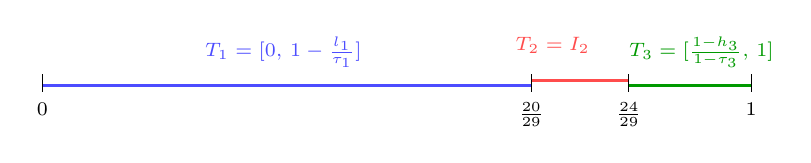
\begin{tikzpicture}[xscale=9,yscale=1]
  \draw[very thick,blue!70]  (0,0)      -- (0.6897,0);
  \draw[very thick,red!70]   (0.6897,0.06) -- (0.8276,0.06);
  \draw[very thick,green!60!black] (0.8276,0) -- (1,0);
  \foreach \x in {0,0.6897,0.8276,1} \draw (\x,-0.08) -- (\x,0.14);
  \node[below,font=\scriptsize] at (0,-0.1) {$0$};
  \node[below,font=\scriptsize] at (0.6897,-0.1) {$\tfrac{20}{29}$};
  \node[below,font=\scriptsize] at (0.8276,-0.1) {$\tfrac{24}{29}$};
  \node[below,font=\scriptsize] at (1,-0.1) {$1$};
  \node[above,font=\scriptsize,blue!70] at (0.34,0.1)
    {$T_1=[0,\,1-\frac{l_1}{\tau_1}]$};
  \node[above,font=\scriptsize,red!70] at (0.72,0.28) {$T_2=I_2$};
  \node[above,font=\scriptsize,green!60!black] at (0.93,0.1)
    {$T_3=[\frac{1-h_3}{1-\tau_3},\,1]$};
\end{tikzpicture}
\caption{The MMM edge tiling on $AB$ (roles $(c,f,g)=(1,2,3)$) for the running
example $\tau=(\tfrac59,\tfrac45,\tfrac16)$: the traces of
$I=([\tfrac5{29},\tfrac{25}{29}],[\tfrac{20}{29},\tfrac{24}{29}],
[\tfrac4{29},\tfrac9{29}])$ abut at $\tfrac{20}{29}$ and $\tfrac{24}{29}$ and
tile $[0,1]$, as forced in Case MMM.}
\label{fig:tiling}
\end{figure}

\subsection*{Case LLL}
All $T_g$ are degenerate, so each edge is tiled by
$T_c=[1-h_c/\tau_c,\,1-l_c/\tau_c]$ (the full image, as $I_c\subset[0,\tau_c]$)
and $T_f=I_f$ with $h_f\le\tau_f<1$. The tile containing $1$ must be $T_c$,
forcing $l_c=0$. If $h_c=\tau_c$ then $T_c=[0,1]$ and $T_f$ has empty interior,
impossible; so $T_f$ contains $0$ ($l_f=0$) and abuts $T_c$:
$h_f=1-h_c/\tau_c$. On the three edges: $l_i=0$ for all $i$, and the $h_i$
satisfy the \emph{same} cyclic system as the $l_i$ in case MMM, so
$h_i=\lambda_i$, giving $\bigl([0,\lambda_i]\bigr)_i$ (type $\mathrm L$ since
$\lambda_i<\tau_i$). Applying the reflection symmetry, the orbit representative
RRR yields the unique solution $h_i=1$, $l_i=\rho_i$, i.e.\
$\bigl([\rho_i,1]\bigr)_i$; equivalently, the $l_i$ satisfy the same cyclic
system as the $h_i$ in case MMM.

\subsection*{Case MML \textup(impossible\textup)}
On $AB$: $T_3$ is degenerate ($I_3$ of type $\mathrm L$), so $[0,1]$ is tiled
by $T_1=[0,\,1-l_1/\tau_1]$ (O1) and $T_2=I_2$. If $1\in T_1$ then $T_1=[0,1]$
and $T_2$ has empty interior, impossible; so $h_2=1$. Then on $BC$ the high
trace \eqref{eq:traces} is
$T_2=[\tfrac{1-h_2}{1-\tau_2},\min(1,\tfrac{1-l_2}{1-\tau_2})]=[0,1]$ (as
$h_2=1$ and $l_2<\tau_2$), leaving the full trace $T_1=I_1$ (positive length)
with empty interior --- contradiction.

\subsection*{Case LLM \textup(impossible\textup)}
On $BC$ ($(c,f,g)=(3,1,2)$): the high trace is degenerate ($I_2$ of type
$\mathrm L$), so $[0,1]$ is tiled by $T_3=[0,\,1-l_3/\tau_3]$ (O1, $I_3$ of
type $\mathrm M$) and $T_1=I_1$ with $h_1\le\tau_1<1$. The tile containing $1$
must be $T_3$, so $l_3=0$ and $T_3=[0,1]$, leaving $T_1$ with empty interior
--- contradiction.

\subsection*{Case LLR \textup(impossible\textup)}
On $BC$ both compressed traces are degenerate ($I_3$ of type $\mathrm R$ gives
a degenerate low trace, $I_2$ of type $\mathrm L$ a degenerate high trace), so
$T_1=I_1$ alone tiles $[0,1]$, forcing $h_1=1>\tau_1$ --- contradicting type
$\mathrm L$.

\subsection*{Case LMR \textup(impossible\textup)}
\emph{On $BC$} ($(c,f,g)=(3,1,2)$): the low trace is degenerate ($I_3$ of type
$\mathrm R$), so $T_1=I_1$ and $T_2=[\tfrac{1-h_2}{1-\tau_2},\,1]$ (O1, $I_2$
of type $\mathrm M$) tile $[0,1]$. If $T_2=[0,1]$ then $T_1$ has empty
interior, impossible; so $T_1$ contains $0$ and abuts $T_2$: $l_1=0$ and
$h_1=\tfrac{1-h_2}{1-\tau_2}$.

\emph{On $CA$} ($(c,f,g)=(2,3,1)$): the high trace is degenerate ($I_1$ of type
$\mathrm L$), so $T_2=[0,\,1-l_2/\tau_2]$ (O1) and $T_3=I_3$ tile $[0,1]$. If
$T_2=[0,1]$ then $T_3$ has empty interior, impossible; so $h_3=1$ and
$l_3=1-l_2/\tau_2$. Since $I_3$ has positive width, $l_3<1$, which forces
$l_2>0$.

\emph{On $AB$} ($(c,f,g)=(1,2,3)$): as $h_3=1$, the high trace is
$T_3=\bigl[0,\,\min\bigl(1,\tfrac{1-l_3}{1-\tau_3}\bigr)\bigr]$. Two subcases.
If $\tfrac{1-l_3}{1-\tau_3}\ge1$, then $T_3=[0,1]$ and the full trace
$T_2=I_2$ (positive length) has empty interior --- contradiction. Otherwise
$T_3=\bigl[0,\,\tfrac{1-l_3}{1-\tau_3}\bigr]
=\bigl[0,\,\tfrac{l_2}{\tau_2(1-\tau_3)}\bigr]$; since $\tau_2(1-\tau_3)<1$
and $l_2>0$, its right endpoint strictly exceeds $l_2$, so the interiors of
$T_3$ and of $T_2=[l_2,h_2]$ overlap on an interval just above $l_2$ ---
contradiction.

\subsection*{Case LRM \textup(impossible\textup)}
On $CA$: both compressed traces are degenerate ($I_2$ of type $\mathrm R$,
$I_1$ of type $\mathrm L$), so $T_3=I_3$ alone tiles $[0,1]$, i.e.\
$I_3=[0,1]$. Then on $AB$ the high trace \eqref{eq:traces} is
$T_3=[\tfrac{1-h_3}{1-\tau_3},\min(1,\tfrac{1-l_3}{1-\tau_3})]=[0,1]$, leaving
$T_2=I_2$ (positive length) with empty interior --- contradiction.

\medskip
All orbits are exhausted, proving Proposition~\ref{prop:tilings}. \qed

\medskip
The three solutions have also been verified by exact rational searches at
$\tau=(\tfrac12,\tfrac12,\tfrac12)$ and $\tau=(\tfrac12,\tfrac23,\tfrac13)$,
and the median enumeration was verified by two further independent exact
computations; all scripts are archived as ancillary files
(Appendix~\ref{app:ancillary}).

\section{Ancillary files and verification protocol}\label{app:ancillary}

This paper is \emph{not} computer-assisted: every theorem is proved in full
in the text or in Appendix~\ref{app:tilings}, and no proof depends on a
computation that is not reproduced in the text. The ancillary scripts are
\emph{secondary verification}: exact re-derivations --- rational or symbolic
arithmetic throughout, never floating point --- of the load-bearing
identities and finite case enumerations, archived so that a reader can
re-check them mechanically. Where a script enumerates cases (tiling types,
role patterns), the enumeration is exhaustive over an explicitly finite index
set, so no case is lost by sampling. For each script we record what it
verifies and which statement it accompanies; all run under Python~3 with
SymPy (or only integer/rational standard libraries where noted).

\begin{itemize}
\item\texttt{median\_rigidity\_enumeration.py} --- exhaustive symbolic
enumeration: the median edge-tiling system has exactly three solutions
(Lemma~\ref{lem:three}).
\item\texttt{median\_edgetilings\_independent.py},
\texttt{median\_edgetiling\_types\_crosscheck.py} --- two independent exact
re-checks of the same enumeration (no SymPy; and via the L/M/R trace
formulas of Appendix~\ref{app:tilings}).
\item\texttt{median\_rigidity\_centroid.py} --- the centroid witness in
Theorem~\ref{thm:median}.
\item\texttt{cyclic\_family\_tight\_rigidity.py} --- Theorem~\ref{thm:tight}:
the identities of Lemma~\ref{lem:margin}, positivity of the witnesses of
Lemma~\ref{lem:witness}, exact coverage checks at several family points, and
the general-$\tau$ solutions of Proposition~\ref{prop:tilings}.
\item\texttt{role\_patterns\_classification.py} --- Theorem~\ref{thm:char}:
exact classification of all $216$ role assignments.
\item\texttt{bang\_Nc\_nogo\_chord.py} --- Proposition~\ref{thm:nogo}: exact
segment tightness of the chord lemma.
\item\texttt{transport\_defect.py} --- \S\ref{sec:defect}: the facet loop
marginals (Theorem~\ref{thm:facetdefect}), exact concurrence defects, the
frozen-weight identities (Theorem~\ref{thm:defectstab}), and the sandwich
example (Remark~\ref{rem:sandwich}).
\item\texttt{defect\_duality.py} --- \S\ref{sec:defect} and
\S\ref{sec:simplex3}: the facet dual certificate, the wedge-certificate
algebra of Proposition~\ref{prop:wedge} (including the sandwich dependency
$c=(75,76,74)$), the sign-counting of Lemma~\ref{lem:external}, the centroid
bound (Theorem~\ref{thm:centroid}), the cycle marginals of
Theorem~\ref{thm:facetd} for $2\le d\le7$, and the region algebra of
Corollary~\ref{cor:region}.
\item\texttt{simplex3\_weighted\_skeleton.py} --- Theorem~\ref{thm:simplex3}
(closed forms $a(\sigma),b(\sigma)$, uniqueness) and
Proposition~\ref{prop:skelobstruction}.
\item\texttt{delta\_eq\_deltac.py} --- Theorem~\ref{thm:deltas} and
Lemma~\ref{lem:external}: the counting lemma on $2928$ exact external
$(q,a)$ samples, and $\delta=\delta_c$ with the exact point-in-triangle test
on a sweep of $507$ triples covering all three full-edge pattern classes.
\item\texttt{supD\_dual\_hunt.py}, \texttt{supD\_hunt\_phase2.py} ---
the multi-knot dual machinery behind Remark~\ref{rem:sandwich}
(float-guided search; every reported bound re-derived exactly), skeleton
upper bounds, and the searches of Problem~\ref{prob:defect}.
\item\texttt{dual\_certificates.py} --- \emph{self-contained} exact
verifier (rational arithmetic, no optimization libraries) of the three
archival certificates of Remark~\ref{rem:sandwich}.
\item\texttt{gardner\_third\_marginal.py} --- the moment obstruction for
pair-witness mixtures (any Gardner witness of two facet directions has
third marginal $\delta_0$), documenting a refuted route to
Problem~\ref{prob:defect}.
\item\texttt{covering\_constant.py} --- Theorem~\ref{thm:canon} (the three
polynomial identities, coverage and margins), the exact coverage oracle
behind the experiments of \S\ref{sec:problems}, and
Remark~\ref{rem:parallelpath}'s symbolic skeleton bound.
\end{itemize}

\begin{thebibliography}{9}
\bibitem{Ambrus} G.\ Ambrus, \emph{Appendix: Plank problems}, manuscript,
2010; available at \texttt{https://users.renyi.hu/\~{}ambrus/appendix.pdf}.
\bibitem{Ball91} K.\ Ball, \emph{The plank problem for symmetric bodies},
Invent.\ Math.\ \textbf{104} (1991), 535--543.
\bibitem{Bang51} T.\ Bang, \emph{A solution of the ``plank problem''},
Proc.\ Amer.\ Math.\ Soc.\ \textbf{2} (1951), 990--993.
\bibitem{BY26} E.\ Bakaev, A.\ Yehudayoff, \emph{A note on the affine plank
conjecture}, arXiv:2602.20290, 2026.
\bibitem{Gardner88} R.\ J.\ Gardner, \emph{Relative width measures and the plank
problem}, Pacific J.\ Math.\ \textbf{135} (1988), no.\ 2, 299--312.
\bibitem{Sion58} M.\ Sion, \emph{On general minimax theorems}, Pacific J.\
Math.\ \textbf{8} (1958), 171--176.
\bibitem{Verreault} W.\ Verreault, \emph{Plank theorems and their applications: a
survey}, arXiv:2203.05540v2, 2025.
\end{thebibliography}
\end{document}
